% Options for packages loaded elsewhere
\PassOptionsToPackage{unicode}{hyperref}
\PassOptionsToPackage{hyphens}{url}
%
\documentclass[
]{book}
\usepackage{amsmath,amssymb}
\usepackage{iftex}
\ifPDFTeX
  \usepackage[T1]{fontenc}
  \usepackage[utf8]{inputenc}
  \usepackage{textcomp} % provide euro and other symbols
\else % if luatex or xetex
  \usepackage{unicode-math} % this also loads fontspec
  \defaultfontfeatures{Scale=MatchLowercase}
  \defaultfontfeatures[\rmfamily]{Ligatures=TeX,Scale=1}
\fi
\usepackage{lmodern}
\ifPDFTeX\else
  % xetex/luatex font selection
\fi
% Use upquote if available, for straight quotes in verbatim environments
\IfFileExists{upquote.sty}{\usepackage{upquote}}{}
\IfFileExists{microtype.sty}{% use microtype if available
  \usepackage[]{microtype}
  \UseMicrotypeSet[protrusion]{basicmath} % disable protrusion for tt fonts
}{}
\makeatletter
\@ifundefined{KOMAClassName}{% if non-KOMA class
  \IfFileExists{parskip.sty}{%
    \usepackage{parskip}
  }{% else
    \setlength{\parindent}{0pt}
    \setlength{\parskip}{6pt plus 2pt minus 1pt}}
}{% if KOMA class
  \KOMAoptions{parskip=half}}
\makeatother
\usepackage{xcolor}
\usepackage{color}
\usepackage{fancyvrb}
\newcommand{\VerbBar}{|}
\newcommand{\VERB}{\Verb[commandchars=\\\{\}]}
\DefineVerbatimEnvironment{Highlighting}{Verbatim}{commandchars=\\\{\}}
% Add ',fontsize=\small' for more characters per line
\usepackage{framed}
\definecolor{shadecolor}{RGB}{248,248,248}
\newenvironment{Shaded}{\begin{snugshade}}{\end{snugshade}}
\newcommand{\AlertTok}[1]{\textcolor[rgb]{0.94,0.16,0.16}{#1}}
\newcommand{\AnnotationTok}[1]{\textcolor[rgb]{0.56,0.35,0.01}{\textbf{\textit{#1}}}}
\newcommand{\AttributeTok}[1]{\textcolor[rgb]{0.13,0.29,0.53}{#1}}
\newcommand{\BaseNTok}[1]{\textcolor[rgb]{0.00,0.00,0.81}{#1}}
\newcommand{\BuiltInTok}[1]{#1}
\newcommand{\CharTok}[1]{\textcolor[rgb]{0.31,0.60,0.02}{#1}}
\newcommand{\CommentTok}[1]{\textcolor[rgb]{0.56,0.35,0.01}{\textit{#1}}}
\newcommand{\CommentVarTok}[1]{\textcolor[rgb]{0.56,0.35,0.01}{\textbf{\textit{#1}}}}
\newcommand{\ConstantTok}[1]{\textcolor[rgb]{0.56,0.35,0.01}{#1}}
\newcommand{\ControlFlowTok}[1]{\textcolor[rgb]{0.13,0.29,0.53}{\textbf{#1}}}
\newcommand{\DataTypeTok}[1]{\textcolor[rgb]{0.13,0.29,0.53}{#1}}
\newcommand{\DecValTok}[1]{\textcolor[rgb]{0.00,0.00,0.81}{#1}}
\newcommand{\DocumentationTok}[1]{\textcolor[rgb]{0.56,0.35,0.01}{\textbf{\textit{#1}}}}
\newcommand{\ErrorTok}[1]{\textcolor[rgb]{0.64,0.00,0.00}{\textbf{#1}}}
\newcommand{\ExtensionTok}[1]{#1}
\newcommand{\FloatTok}[1]{\textcolor[rgb]{0.00,0.00,0.81}{#1}}
\newcommand{\FunctionTok}[1]{\textcolor[rgb]{0.13,0.29,0.53}{\textbf{#1}}}
\newcommand{\ImportTok}[1]{#1}
\newcommand{\InformationTok}[1]{\textcolor[rgb]{0.56,0.35,0.01}{\textbf{\textit{#1}}}}
\newcommand{\KeywordTok}[1]{\textcolor[rgb]{0.13,0.29,0.53}{\textbf{#1}}}
\newcommand{\NormalTok}[1]{#1}
\newcommand{\OperatorTok}[1]{\textcolor[rgb]{0.81,0.36,0.00}{\textbf{#1}}}
\newcommand{\OtherTok}[1]{\textcolor[rgb]{0.56,0.35,0.01}{#1}}
\newcommand{\PreprocessorTok}[1]{\textcolor[rgb]{0.56,0.35,0.01}{\textit{#1}}}
\newcommand{\RegionMarkerTok}[1]{#1}
\newcommand{\SpecialCharTok}[1]{\textcolor[rgb]{0.81,0.36,0.00}{\textbf{#1}}}
\newcommand{\SpecialStringTok}[1]{\textcolor[rgb]{0.31,0.60,0.02}{#1}}
\newcommand{\StringTok}[1]{\textcolor[rgb]{0.31,0.60,0.02}{#1}}
\newcommand{\VariableTok}[1]{\textcolor[rgb]{0.00,0.00,0.00}{#1}}
\newcommand{\VerbatimStringTok}[1]{\textcolor[rgb]{0.31,0.60,0.02}{#1}}
\newcommand{\WarningTok}[1]{\textcolor[rgb]{0.56,0.35,0.01}{\textbf{\textit{#1}}}}
\usepackage{longtable,booktabs,array}
\usepackage{calc} % for calculating minipage widths
% Correct order of tables after \paragraph or \subparagraph
\usepackage{etoolbox}
\makeatletter
\patchcmd\longtable{\par}{\if@noskipsec\mbox{}\fi\par}{}{}
\makeatother
% Allow footnotes in longtable head/foot
\IfFileExists{footnotehyper.sty}{\usepackage{footnotehyper}}{\usepackage{footnote}}
\makesavenoteenv{longtable}
\usepackage{graphicx}
\makeatletter
\def\maxwidth{\ifdim\Gin@nat@width>\linewidth\linewidth\else\Gin@nat@width\fi}
\def\maxheight{\ifdim\Gin@nat@height>\textheight\textheight\else\Gin@nat@height\fi}
\makeatother
% Scale images if necessary, so that they will not overflow the page
% margins by default, and it is still possible to overwrite the defaults
% using explicit options in \includegraphics[width, height, ...]{}
\setkeys{Gin}{width=\maxwidth,height=\maxheight,keepaspectratio}
% Set default figure placement to htbp
\makeatletter
\def\fps@figure{htbp}
\makeatother
\setlength{\emergencystretch}{3em} % prevent overfull lines
\providecommand{\tightlist}{%
  \setlength{\itemsep}{0pt}\setlength{\parskip}{0pt}}
\setcounter{secnumdepth}{5}
\ifLuaTeX
  \usepackage{selnolig}  % disable illegal ligatures
\fi
\usepackage[]{natbib}
\bibliographystyle{apalike}
\nocite{*}
\IfFileExists{bookmark.sty}{\usepackage{bookmark}}{\usepackage{hyperref}}
\IfFileExists{xurl.sty}{\usepackage{xurl}}{} % add URL line breaks if available
\urlstyle{same}
\hypersetup{
  pdftitle={Supplemental Material for `Lexidate: Model Evaluation and Selection with Lexicase Selection'},
  pdfauthor={Anonymous GECCO},
  hidelinks,
  pdfcreator={LaTeX via pandoc}}

\title{Supplemental Material for `Lexidate: Model Evaluation and Selection with Lexicase Selection'}
\author{Anonymous GECCO}
\date{2024-01-31}

\begin{document}
\maketitle

{
\setcounter{tocdepth}{1}
\tableofcontents
}
\begin{Shaded}
\begin{Highlighting}[]
\FunctionTok{library}\NormalTok{(ggplot2)}
\FunctionTok{library}\NormalTok{(cowplot)}
\FunctionTok{library}\NormalTok{(dplyr)}
\FunctionTok{library}\NormalTok{(PupillometryR)}
\FunctionTok{library}\NormalTok{(scales) }\CommentTok{\# to access break formatting functions}


\NormalTok{NAMES }\OtherTok{\textless{}{-}} \FunctionTok{c}\NormalTok{(}\StringTok{"10{-}fold cv"}\NormalTok{,}\StringTok{"90/10"}\NormalTok{,}\StringTok{"70/30"}\NormalTok{,}\StringTok{"50/50"}\NormalTok{)}
\NormalTok{SHAPE }\OtherTok{\textless{}{-}} \FunctionTok{c}\NormalTok{(}\DecValTok{21}\NormalTok{,}\DecValTok{24}\NormalTok{,}\DecValTok{22}\NormalTok{,}\DecValTok{25}\NormalTok{)}
\NormalTok{cb\_palette }\OtherTok{\textless{}{-}} \FunctionTok{c}\NormalTok{(}\StringTok{\textquotesingle{}\#D81B60\textquotesingle{}}\NormalTok{,}\StringTok{\textquotesingle{}\#1E88E5\textquotesingle{}}\NormalTok{,}\StringTok{\textquotesingle{}\#FFC107\textquotesingle{}}\NormalTok{,}\StringTok{\textquotesingle{}\#004D40\textquotesingle{}}\NormalTok{)}
\NormalTok{TSIZE }\OtherTok{\textless{}{-}} \DecValTok{22}
\NormalTok{task\_id\_lists }\OtherTok{\textless{}{-}} \FunctionTok{c}\NormalTok{(}\DecValTok{167104}\NormalTok{, }\DecValTok{167184}\NormalTok{, }\DecValTok{167168}\NormalTok{, }\DecValTok{167161}\NormalTok{, }\DecValTok{167185}\NormalTok{, }\DecValTok{189905}\NormalTok{)}

\NormalTok{p\_theme }\OtherTok{\textless{}{-}} \FunctionTok{theme}\NormalTok{(}
  \AttributeTok{plot.title =} \FunctionTok{element\_text}\NormalTok{( }\AttributeTok{face =} \StringTok{"bold"}\NormalTok{, }\AttributeTok{size =} \DecValTok{22}\NormalTok{, }\AttributeTok{hjust=}\FloatTok{0.5}\NormalTok{),}
  \AttributeTok{panel.border =} \FunctionTok{element\_blank}\NormalTok{(),}
  \AttributeTok{panel.grid.minor =} \FunctionTok{element\_blank}\NormalTok{(),}
  \AttributeTok{legend.title=}\FunctionTok{element\_text}\NormalTok{(}\AttributeTok{size=}\DecValTok{20}\NormalTok{),}
  \AttributeTok{legend.text=}\FunctionTok{element\_text}\NormalTok{(}\AttributeTok{size=}\DecValTok{20}\NormalTok{),}
  \AttributeTok{axis.title =} \FunctionTok{element\_text}\NormalTok{(}\AttributeTok{size=}\DecValTok{20}\NormalTok{),}
  \AttributeTok{axis.text =} \FunctionTok{element\_text}\NormalTok{(}\AttributeTok{size=}\DecValTok{19}\NormalTok{),}
  \AttributeTok{legend.position=}\StringTok{"bottom"}\NormalTok{,}
  \AttributeTok{panel.background =} \FunctionTok{element\_rect}\NormalTok{(}\AttributeTok{fill =} \StringTok{"\#f1f2f5"}\NormalTok{,}
                                  \AttributeTok{colour =} \StringTok{"white"}\NormalTok{,}
                                  \AttributeTok{size =} \FloatTok{0.5}\NormalTok{, }\AttributeTok{linetype =} \StringTok{"solid"}\NormalTok{)}
\NormalTok{)}
\end{Highlighting}
\end{Shaded}

\hypertarget{introduction}{%
\chapter{Introduction}\label{introduction}}

This is not intended as a stand-alone document, but as a companion to our manuscript.

\hypertarget{about-our-supplemental-material}{%
\section{About our supplemental material}\label{about-our-supplemental-material}}

As you may have noticed (unless you're reading a pdf version of this), our supplemental material is hosted using \href{https://pages.github.com/}{GitHub pages}.
We compiled our data analyses and supplemental documentation into this nifty web-accessible book using \href{https://bookdown.org}{bookdown}.

The code used for this supplemental material can be found in \href{https://github.com/jgh9094/GECCO-2024-LEXIDATE-EVALUATION}{this GitHub repository}.

Our supplemental material includes the following:

\begin{itemize}
\tightlist
\item
  Accuracy results (Section \ref{accuracy-results})
\item
  Complexity results (Section \ref{complexity-results})
\end{itemize}

\hypertarget{contributing-authors}{%
\section{Contributing authors}\label{contributing-authors}}

\begin{itemize}
\tightlist
\item
  \href{https://jgh9094.github.io/}{Jose Guadalupe Hernandez}
\item
  \href{https://theaksaini.github.io/}{Anil Kumar Saini}
\item
  \href{https://jasonhmoore.org/}{Jason H. Moore}
\end{itemize}

\hypertarget{accuracy-results}{%
\chapter{Accuracy results}\label{accuracy-results}}

Here we report the accuracy for \textbf{final pipeline returned from a TPOT2 run} on each OpenML task.
40 replicates were conducted for each evaluation strategy explored.

\hypertarget{analysis-setup}{%
\section{Analysis setup}\label{analysis-setup}}

\begin{Shaded}
\begin{Highlighting}[]
\FunctionTok{library}\NormalTok{(ggplot2)}
\FunctionTok{library}\NormalTok{(cowplot)}
\FunctionTok{library}\NormalTok{(dplyr)}
\FunctionTok{library}\NormalTok{(PupillometryR)}

\NormalTok{scores }\OtherTok{\textless{}{-}} \FunctionTok{read.csv}\NormalTok{(}\StringTok{"./scores.csv"}\NormalTok{, }\AttributeTok{header =} \ConstantTok{TRUE}\NormalTok{, }\AttributeTok{stringsAsFactors =} \ConstantTok{FALSE}\NormalTok{)}
\NormalTok{scores}\SpecialCharTok{$}\NormalTok{acro }\OtherTok{\textless{}{-}} \FunctionTok{factor}\NormalTok{(scores}\SpecialCharTok{$}\NormalTok{acro, }\AttributeTok{levels =}\NormalTok{ NAMES)}
\end{Highlighting}
\end{Shaded}

\hypertarget{accuracy-per-openml-task}{%
\section{Accuracy per OpenML task}\label{accuracy-per-openml-task}}

Accuracy of the returned pipeline from an evolutionary run.

\hypertarget{task-167104}{%
\subsection{Task 167104}\label{task-167104}}

\begin{Shaded}
\begin{Highlighting}[]
\FunctionTok{filter}\NormalTok{(scores, taskid }\SpecialCharTok{==}\NormalTok{ task\_id\_lists[}\DecValTok{1}\NormalTok{]) }\SpecialCharTok{\%\textgreater{}\%}
  \FunctionTok{ggplot}\NormalTok{(., }\FunctionTok{aes}\NormalTok{(}\AttributeTok{x =}\NormalTok{ acro, }\AttributeTok{y =}\NormalTok{ accuracy, }\AttributeTok{color =}\NormalTok{ acro,}
                \AttributeTok{fill =}\NormalTok{ acro, }\AttributeTok{shape =}\NormalTok{ acro)) }\SpecialCharTok{+}
  \FunctionTok{geom\_flat\_violin}\NormalTok{(}\AttributeTok{position =} \FunctionTok{position\_nudge}\NormalTok{(}\AttributeTok{x =} \FloatTok{0.1}\NormalTok{, }\AttributeTok{y =} \DecValTok{0}\NormalTok{),}
                   \AttributeTok{scale =} \StringTok{"width"}\NormalTok{, }\AttributeTok{alpha =} \FloatTok{0.2}\NormalTok{, }\AttributeTok{width =} \FloatTok{1.5}\NormalTok{) }\SpecialCharTok{+}
  \FunctionTok{geom\_boxplot}\NormalTok{(}\AttributeTok{color =} \StringTok{"black"}\NormalTok{, }\AttributeTok{width =}\NormalTok{ .}\DecValTok{08}\NormalTok{, }\AttributeTok{outlier.shape =} \ConstantTok{NA}\NormalTok{, }\AttributeTok{alpha =} \FloatTok{0.0}\NormalTok{,}
               \AttributeTok{size =} \FloatTok{0.8}\NormalTok{, }\AttributeTok{position =} \FunctionTok{position\_nudge}\NormalTok{(}\AttributeTok{x =}\NormalTok{ .}\DecValTok{15}\NormalTok{, }\AttributeTok{y =} \DecValTok{0}\NormalTok{)) }\SpecialCharTok{+}
  \FunctionTok{geom\_point}\NormalTok{(}\AttributeTok{position =} \FunctionTok{position\_jitter}\NormalTok{(}\AttributeTok{width =}\NormalTok{ .}\DecValTok{015}\NormalTok{, }\AttributeTok{height =}\NormalTok{ .}\DecValTok{0001}\NormalTok{),}
             \AttributeTok{size =} \FloatTok{2.0}\NormalTok{, }\AttributeTok{alpha =} \FloatTok{1.0}\NormalTok{) }\SpecialCharTok{+}
  \FunctionTok{scale\_y\_continuous}\NormalTok{(}
    \AttributeTok{name =} \StringTok{"Accuracy \%"}\NormalTok{,}
    \AttributeTok{breaks =} \FunctionTok{c}\NormalTok{(.}\DecValTok{74}\NormalTok{, .}\DecValTok{78}\NormalTok{, .}\DecValTok{82}\NormalTok{, .}\DecValTok{86}\NormalTok{),}
    \AttributeTok{labels =}\NormalTok{ scales}\SpecialCharTok{::}\NormalTok{percent}

\NormalTok{  ) }\SpecialCharTok{+}
  \FunctionTok{scale\_x\_discrete}\NormalTok{(}
    \AttributeTok{name =} \StringTok{"Treatment"}
\NormalTok{  ) }\SpecialCharTok{+}
  \FunctionTok{scale\_shape\_manual}\NormalTok{(}\AttributeTok{values =}\NormalTok{ SHAPE,) }\SpecialCharTok{+}
  \FunctionTok{scale\_colour\_manual}\NormalTok{(}\AttributeTok{values =}\NormalTok{ cb\_palette,) }\SpecialCharTok{+}
  \FunctionTok{scale\_fill\_manual}\NormalTok{(}\AttributeTok{values =}\NormalTok{ cb\_palette,) }\SpecialCharTok{+}
  \FunctionTok{ggtitle}\NormalTok{(}\StringTok{"Accuracy"}\NormalTok{) }\SpecialCharTok{+}
\NormalTok{  p\_theme }\SpecialCharTok{+}
  \FunctionTok{guides}\NormalTok{(}
    \AttributeTok{shape=}\FunctionTok{guide\_legend}\NormalTok{(}\AttributeTok{nrow =} \DecValTok{1}\NormalTok{, }\AttributeTok{title.position =} \StringTok{"bottom"}\NormalTok{,}
                       \AttributeTok{title =} \StringTok{"Evaluation strategy"}\NormalTok{),}
    \AttributeTok{color=}\FunctionTok{guide\_legend}\NormalTok{(}\AttributeTok{nrow =} \DecValTok{1}\NormalTok{, }\AttributeTok{title.position =} \StringTok{"bottom"}\NormalTok{,}
                       \AttributeTok{title =} \StringTok{"Evaluation strategy"}\NormalTok{),}
    \AttributeTok{fill=}\FunctionTok{guide\_legend}\NormalTok{(}\AttributeTok{nrow =} \DecValTok{1}\NormalTok{, }\AttributeTok{title.position =} \StringTok{"bottom"}\NormalTok{,}
                      \AttributeTok{title =} \StringTok{"Evaluation strategy"}\NormalTok{)}
\NormalTok{  )}
\end{Highlighting}
\end{Shaded}

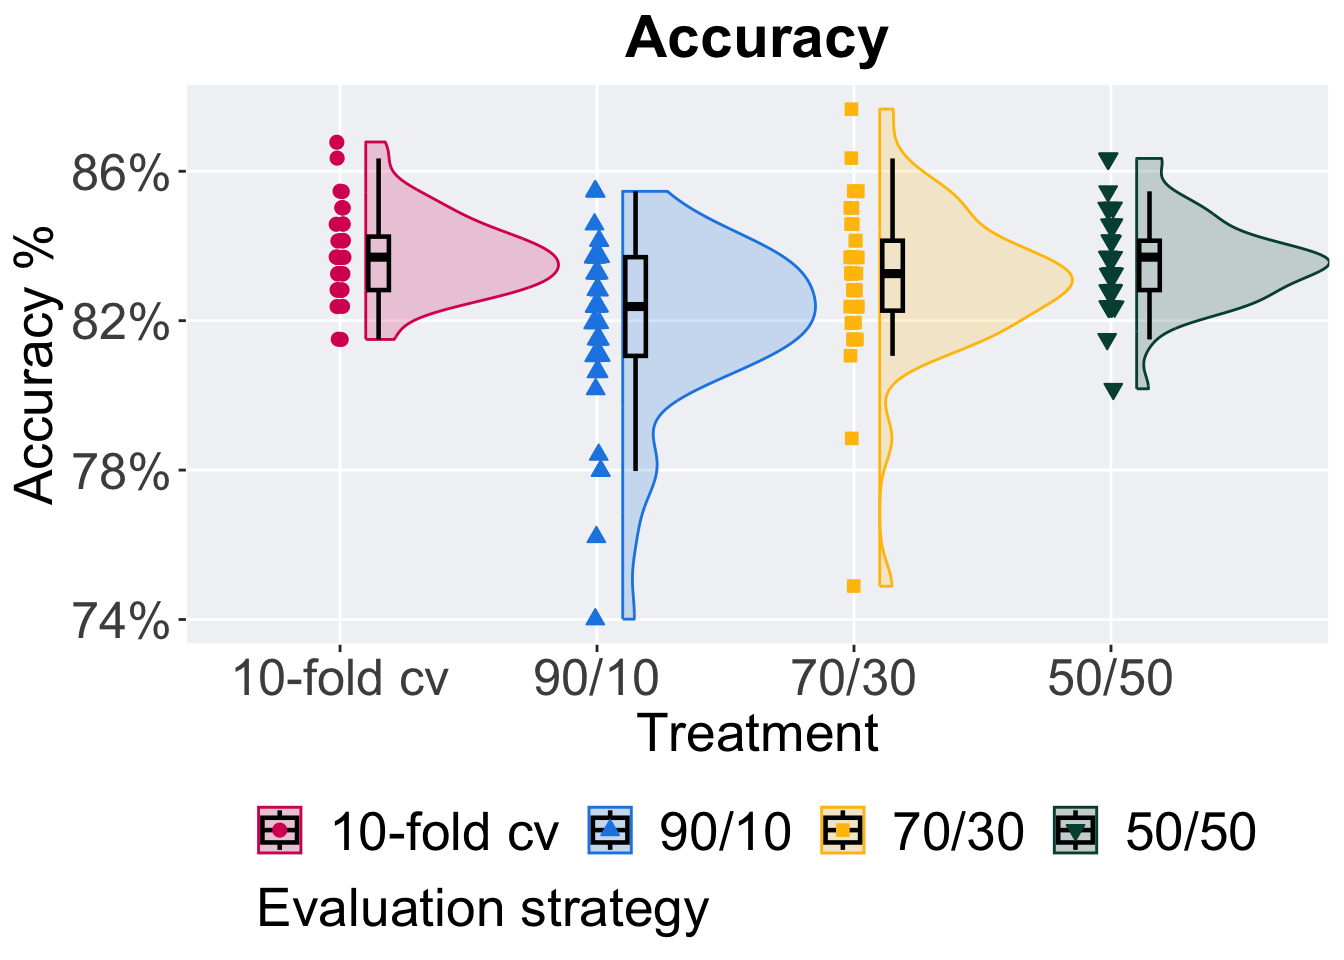
\includegraphics[width=1\linewidth]{lexidate-validation-supplemental_files/figure-latex/acc-task-1-plt-1}

Summary statistics for the generation a satisfactory solution is found.

\begin{Shaded}
\begin{Highlighting}[]
\NormalTok{performance }\OtherTok{\textless{}{-}} \FunctionTok{filter}\NormalTok{(scores, taskid }\SpecialCharTok{==}\NormalTok{ task\_id\_lists[}\DecValTok{1}\NormalTok{])}
\NormalTok{performance }\SpecialCharTok{\%\textgreater{}\%}
  \FunctionTok{group\_by}\NormalTok{(acro) }\SpecialCharTok{\%\textgreater{}\%}
\NormalTok{  dplyr}\SpecialCharTok{::}\FunctionTok{summarise}\NormalTok{(}
    \AttributeTok{count =} \FunctionTok{n}\NormalTok{(),}
    \AttributeTok{na\_cnt =} \FunctionTok{sum}\NormalTok{(}\FunctionTok{is.na}\NormalTok{(accuracy)),}
    \AttributeTok{min =} \FunctionTok{min}\NormalTok{(accuracy, }\AttributeTok{na.rm =} \ConstantTok{TRUE}\NormalTok{),}
    \AttributeTok{median =} \FunctionTok{median}\NormalTok{(accuracy, }\AttributeTok{na.rm =} \ConstantTok{TRUE}\NormalTok{),}
    \AttributeTok{mean =} \FunctionTok{mean}\NormalTok{(accuracy, }\AttributeTok{na.rm =} \ConstantTok{TRUE}\NormalTok{),}
    \AttributeTok{max =} \FunctionTok{max}\NormalTok{(accuracy, }\AttributeTok{na.rm =} \ConstantTok{TRUE}\NormalTok{),}
    \AttributeTok{IQR =} \FunctionTok{IQR}\NormalTok{(accuracy, }\AttributeTok{na.rm =} \ConstantTok{TRUE}\NormalTok{)}
\NormalTok{  )}
\end{Highlighting}
\end{Shaded}

\begin{verbatim}
## # A tibble: 4 x 8
##   acro       count na_cnt   min median  mean   max    IQR
##   <fct>      <int>  <int> <dbl>  <dbl> <dbl> <dbl>  <dbl>
## 1 10-fold cv    40      0 0.815  0.837 0.838 0.868 0.0143
## 2 90/10         40      0 0.740  0.824 0.819 0.855 0.0264
## 3 70/30         40      0 0.749  0.833 0.831 0.877 0.0187
## 4 50/50         40      0 0.802  0.837 0.836 0.863 0.0132
\end{verbatim}

Kruskal--Wallis test illustrates evidence of statistical differences.

\begin{Shaded}
\begin{Highlighting}[]
\FunctionTok{kruskal.test}\NormalTok{(accuracy }\SpecialCharTok{\textasciitilde{}}\NormalTok{ acro, }\AttributeTok{data =}\NormalTok{ performance)}
\end{Highlighting}
\end{Shaded}

\begin{verbatim}
## 
##  Kruskal-Wallis rank sum test
## 
## data:  accuracy by acro
## Kruskal-Wallis chi-squared = 21.695, df = 3, p-value = 7.55e-05
\end{verbatim}

Results for post-hoc Wilcoxon rank-sum test with a Bonferroni correction.

\begin{Shaded}
\begin{Highlighting}[]
\FunctionTok{pairwise.wilcox.test}\NormalTok{(}\AttributeTok{x =}\NormalTok{ performance}\SpecialCharTok{$}\NormalTok{accuracy, }\AttributeTok{g =}\NormalTok{ performance}\SpecialCharTok{$}\NormalTok{acro,}
                     \AttributeTok{p.adjust.method =} \StringTok{"bonferroni"}\NormalTok{,}
                     \AttributeTok{paired =} \ConstantTok{FALSE}\NormalTok{, }\AttributeTok{conf.int =} \ConstantTok{FALSE}\NormalTok{, }\AttributeTok{alternative =} \StringTok{"t"}\NormalTok{)}
\end{Highlighting}
\end{Shaded}

\begin{verbatim}
## 
##  Pairwise comparisons using Wilcoxon rank sum test with continuity correction 
## 
## data:  performance$accuracy and performance$acro 
## 
##       10-fold cv 90/10   70/30  
## 90/10 0.00016    -       -      
## 70/30 0.41651    0.08840 -      
## 50/50 1.00000    0.00111 1.00000
## 
## P value adjustment method: bonferroni
\end{verbatim}

\hypertarget{task-167184}{%
\subsection{Task 167184}\label{task-167184}}

\begin{Shaded}
\begin{Highlighting}[]
\FunctionTok{filter}\NormalTok{(scores, taskid }\SpecialCharTok{==}\NormalTok{ task\_id\_lists[}\DecValTok{2}\NormalTok{]) }\SpecialCharTok{\%\textgreater{}\%}
  \FunctionTok{ggplot}\NormalTok{(., }\FunctionTok{aes}\NormalTok{(}\AttributeTok{x =}\NormalTok{ acro, }\AttributeTok{y =}\NormalTok{ accuracy, }\AttributeTok{color =}\NormalTok{ acro,}
                \AttributeTok{fill =}\NormalTok{ acro, }\AttributeTok{shape =}\NormalTok{ acro)) }\SpecialCharTok{+}
  \FunctionTok{geom\_flat\_violin}\NormalTok{(}\AttributeTok{position =} \FunctionTok{position\_nudge}\NormalTok{(}\AttributeTok{x =} \FloatTok{0.1}\NormalTok{, }\AttributeTok{y =} \DecValTok{0}\NormalTok{),}
                   \AttributeTok{scale =} \StringTok{"width"}\NormalTok{, }\AttributeTok{alpha =} \FloatTok{0.2}\NormalTok{, }\AttributeTok{width =} \FloatTok{1.5}\NormalTok{) }\SpecialCharTok{+}
  \FunctionTok{geom\_boxplot}\NormalTok{(}\AttributeTok{color =} \StringTok{"black"}\NormalTok{, }\AttributeTok{width =}\NormalTok{ .}\DecValTok{08}\NormalTok{, }\AttributeTok{outlier.shape =} \ConstantTok{NA}\NormalTok{, }\AttributeTok{alpha =} \FloatTok{0.0}\NormalTok{,}
               \AttributeTok{size =} \FloatTok{0.8}\NormalTok{, }\AttributeTok{position =} \FunctionTok{position\_nudge}\NormalTok{(}\AttributeTok{x =}\NormalTok{ .}\DecValTok{15}\NormalTok{, }\AttributeTok{y =} \DecValTok{0}\NormalTok{)) }\SpecialCharTok{+}
  \FunctionTok{geom\_point}\NormalTok{(}\AttributeTok{position =} \FunctionTok{position\_jitter}\NormalTok{(}\AttributeTok{width =}\NormalTok{ .}\DecValTok{015}\NormalTok{, }\AttributeTok{height =}\NormalTok{ .}\DecValTok{0001}\NormalTok{),}
             \AttributeTok{size =} \FloatTok{2.0}\NormalTok{, }\AttributeTok{alpha =} \FloatTok{1.0}\NormalTok{) }\SpecialCharTok{+}
  \FunctionTok{scale\_y\_continuous}\NormalTok{(}
    \AttributeTok{name =} \StringTok{"Accuracy \%"}\NormalTok{,}
    \AttributeTok{limits=}\FunctionTok{c}\NormalTok{(.}\DecValTok{6}\NormalTok{, .}\DecValTok{9}\NormalTok{),}
    \AttributeTok{labels =}\NormalTok{ scales}\SpecialCharTok{::}\NormalTok{percent}

\NormalTok{  ) }\SpecialCharTok{+}
  \FunctionTok{scale\_x\_discrete}\NormalTok{(}
    \AttributeTok{name =} \StringTok{"Treatment"}
\NormalTok{  ) }\SpecialCharTok{+}
  \FunctionTok{scale\_shape\_manual}\NormalTok{(}\AttributeTok{values =}\NormalTok{ SHAPE) }\SpecialCharTok{+}
  \FunctionTok{scale\_colour\_manual}\NormalTok{(}\AttributeTok{values =}\NormalTok{ cb\_palette, ) }\SpecialCharTok{+}
  \FunctionTok{scale\_fill\_manual}\NormalTok{(}\AttributeTok{values =}\NormalTok{ cb\_palette) }\SpecialCharTok{+}
  \FunctionTok{ggtitle}\NormalTok{(}\StringTok{"Accuracy"}\NormalTok{) }\SpecialCharTok{+}
\NormalTok{  p\_theme }\SpecialCharTok{+}
  \FunctionTok{guides}\NormalTok{(}
    \AttributeTok{shape=}\FunctionTok{guide\_legend}\NormalTok{(}\AttributeTok{nrow =} \DecValTok{1}\NormalTok{, }\AttributeTok{title.position =} \StringTok{"bottom"}\NormalTok{,}
                       \AttributeTok{title =} \StringTok{"Evaluation strategy"}\NormalTok{),}
    \AttributeTok{color=}\FunctionTok{guide\_legend}\NormalTok{(}\AttributeTok{nrow =} \DecValTok{1}\NormalTok{, }\AttributeTok{title.position =} \StringTok{"bottom"}\NormalTok{,}
                       \AttributeTok{title =} \StringTok{"Evaluation strategy"}\NormalTok{),}
    \AttributeTok{fill=}\FunctionTok{guide\_legend}\NormalTok{(}\AttributeTok{nrow =} \DecValTok{1}\NormalTok{, }\AttributeTok{title.position =} \StringTok{"bottom"}\NormalTok{,}
                      \AttributeTok{title =} \StringTok{"Evaluation strategy"}\NormalTok{)}
\NormalTok{  )}
\end{Highlighting}
\end{Shaded}

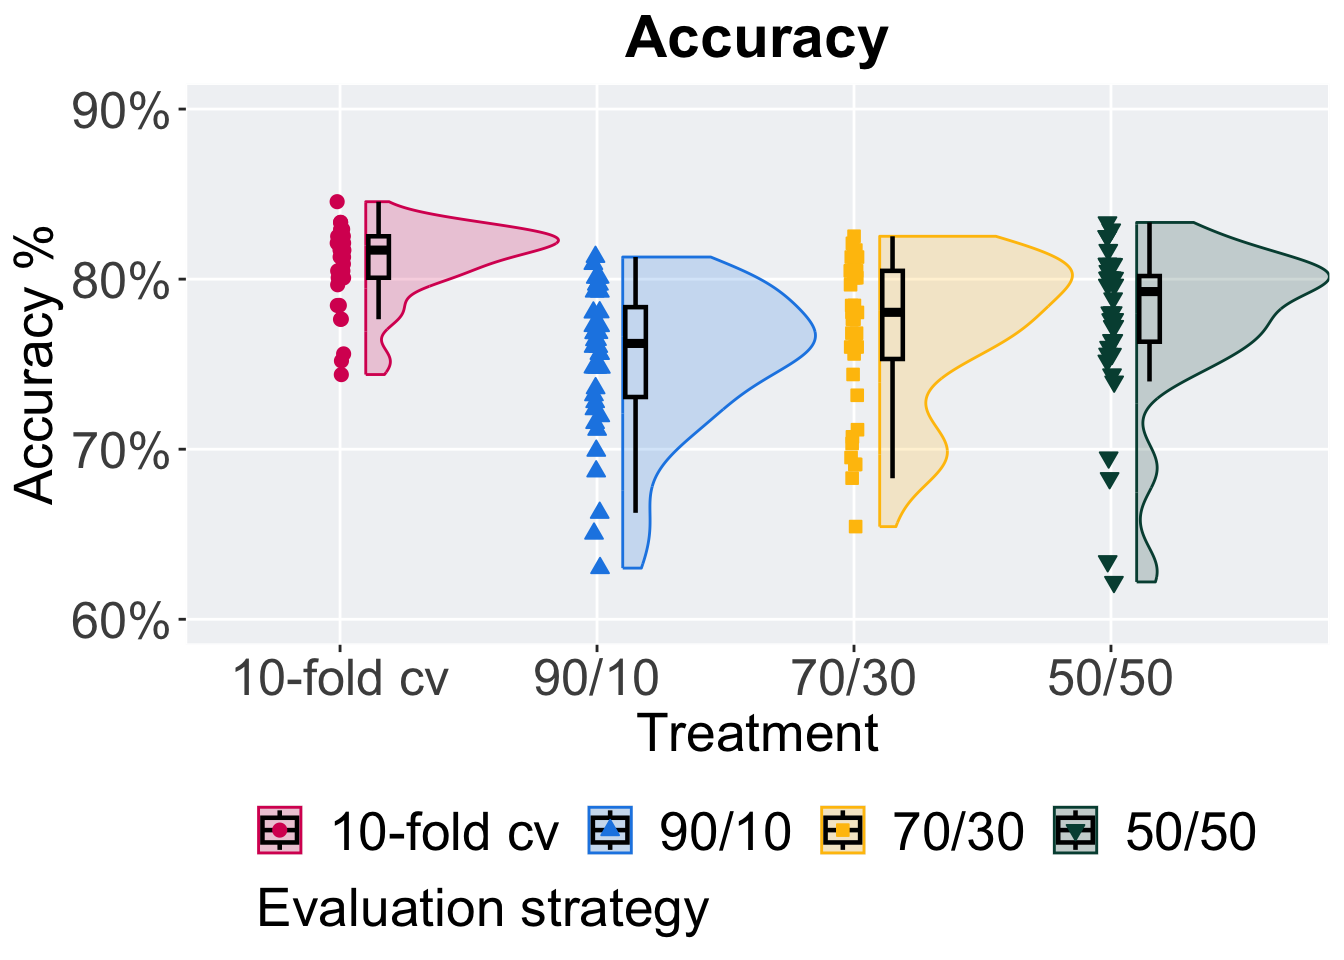
\includegraphics[width=1\linewidth]{lexidate-validation-supplemental_files/figure-latex/acc-task-2-plt-1}

Summary statistics for the generation a satisfactory solution is found.

\begin{Shaded}
\begin{Highlighting}[]
\NormalTok{performance }\OtherTok{\textless{}{-}} \FunctionTok{filter}\NormalTok{(scores, taskid }\SpecialCharTok{==}\NormalTok{ task\_id\_lists[}\DecValTok{2}\NormalTok{])}
\NormalTok{performance }\SpecialCharTok{\%\textgreater{}\%}
  \FunctionTok{group\_by}\NormalTok{(acro) }\SpecialCharTok{\%\textgreater{}\%}
\NormalTok{  dplyr}\SpecialCharTok{::}\FunctionTok{summarise}\NormalTok{(}
    \AttributeTok{count =} \FunctionTok{n}\NormalTok{(),}
    \AttributeTok{na\_cnt =} \FunctionTok{sum}\NormalTok{(}\FunctionTok{is.na}\NormalTok{(accuracy)),}
    \AttributeTok{min =} \FunctionTok{min}\NormalTok{(accuracy, }\AttributeTok{na.rm =} \ConstantTok{TRUE}\NormalTok{),}
    \AttributeTok{median =} \FunctionTok{median}\NormalTok{(accuracy, }\AttributeTok{na.rm =} \ConstantTok{TRUE}\NormalTok{),}
    \AttributeTok{mean =} \FunctionTok{mean}\NormalTok{(accuracy, }\AttributeTok{na.rm =} \ConstantTok{TRUE}\NormalTok{),}
    \AttributeTok{max =} \FunctionTok{max}\NormalTok{(accuracy, }\AttributeTok{na.rm =} \ConstantTok{TRUE}\NormalTok{),}
    \AttributeTok{IQR =} \FunctionTok{IQR}\NormalTok{(accuracy, }\AttributeTok{na.rm =} \ConstantTok{TRUE}\NormalTok{)}
\NormalTok{  )}
\end{Highlighting}
\end{Shaded}

\begin{verbatim}
## # A tibble: 4 x 8
##   acro       count na_cnt   min median  mean   max    IQR
##   <fct>      <int>  <int> <dbl>  <dbl> <dbl> <dbl>  <dbl>
## 1 10-fold cv    40      0 0.744  0.817 0.810 0.846 0.0244
## 2 90/10         40      0 0.630  0.762 0.753 0.813 0.0528
## 3 70/30         40      0 0.654  0.780 0.770 0.825 0.0518
## 4 50/50         40      0 0.622  0.793 0.777 0.833 0.0386
\end{verbatim}

Kruskal--Wallis test illustrates evidence of statistical differences.

\begin{Shaded}
\begin{Highlighting}[]
\FunctionTok{kruskal.test}\NormalTok{(accuracy }\SpecialCharTok{\textasciitilde{}}\NormalTok{ acro, }\AttributeTok{data =}\NormalTok{ performance)}
\end{Highlighting}
\end{Shaded}

\begin{verbatim}
## 
##  Kruskal-Wallis rank sum test
## 
## data:  accuracy by acro
## Kruskal-Wallis chi-squared = 47.311, df = 3, p-value = 2.984e-10
\end{verbatim}

Results for post-hoc Wilcoxon rank-sum test with a Bonferroni correction.

\begin{Shaded}
\begin{Highlighting}[]
\FunctionTok{pairwise.wilcox.test}\NormalTok{(}\AttributeTok{x =}\NormalTok{ performance}\SpecialCharTok{$}\NormalTok{accuracy, }\AttributeTok{g =}\NormalTok{ performance}\SpecialCharTok{$}\NormalTok{acro,}
                     \AttributeTok{p.adjust.method =} \StringTok{"bonferroni"}\NormalTok{,}
                     \AttributeTok{paired =} \ConstantTok{FALSE}\NormalTok{, }\AttributeTok{conf.int =} \ConstantTok{FALSE}\NormalTok{, }\AttributeTok{alternative =} \StringTok{"t"}\NormalTok{)}
\end{Highlighting}
\end{Shaded}

\begin{verbatim}
## 
##  Pairwise comparisons using Wilcoxon rank sum test with continuity correction 
## 
## data:  performance$accuracy and performance$acro 
## 
##       10-fold cv 90/10   70/30  
## 90/10 1.7e-09    -       -      
## 70/30 1.3e-05    0.16648 -      
## 50/50 0.00016    0.01281 1.00000
## 
## P value adjustment method: bonferroni
\end{verbatim}

\hypertarget{task-167168}{%
\subsection{Task 167168}\label{task-167168}}

\begin{Shaded}
\begin{Highlighting}[]
\FunctionTok{filter}\NormalTok{(scores, taskid }\SpecialCharTok{==}\NormalTok{ task\_id\_lists[}\DecValTok{3}\NormalTok{]) }\SpecialCharTok{\%\textgreater{}\%}
  \FunctionTok{ggplot}\NormalTok{(., }\FunctionTok{aes}\NormalTok{(}\AttributeTok{x =}\NormalTok{ acro, }\AttributeTok{y =}\NormalTok{ accuracy, }\AttributeTok{color =}\NormalTok{ acro,}
                \AttributeTok{fill =}\NormalTok{ acro, }\AttributeTok{shape =}\NormalTok{ acro)) }\SpecialCharTok{+}
  \FunctionTok{geom\_flat\_violin}\NormalTok{(}\AttributeTok{position =} \FunctionTok{position\_nudge}\NormalTok{(}\AttributeTok{x =} \FloatTok{0.1}\NormalTok{, }\AttributeTok{y =} \DecValTok{0}\NormalTok{),}
                   \AttributeTok{scale =} \StringTok{"width"}\NormalTok{, }\AttributeTok{alpha =} \FloatTok{0.2}\NormalTok{, }\AttributeTok{width =} \FloatTok{1.5}\NormalTok{) }\SpecialCharTok{+}
  \FunctionTok{geom\_boxplot}\NormalTok{(}\AttributeTok{color =} \StringTok{"black"}\NormalTok{, }\AttributeTok{width =}\NormalTok{ .}\DecValTok{08}\NormalTok{, }\AttributeTok{outlier.shape =} \ConstantTok{NA}\NormalTok{, }\AttributeTok{alpha =} \FloatTok{0.0}\NormalTok{,}
               \AttributeTok{size =} \FloatTok{0.8}\NormalTok{, }\AttributeTok{position =} \FunctionTok{position\_nudge}\NormalTok{(}\AttributeTok{x =}\NormalTok{ .}\DecValTok{15}\NormalTok{, }\AttributeTok{y =} \DecValTok{0}\NormalTok{)) }\SpecialCharTok{+}
  \FunctionTok{geom\_point}\NormalTok{(}\AttributeTok{position =} \FunctionTok{position\_jitter}\NormalTok{(}\AttributeTok{width =}\NormalTok{ .}\DecValTok{015}\NormalTok{, }\AttributeTok{height =}\NormalTok{ .}\DecValTok{0001}\NormalTok{),}
             \AttributeTok{size =} \FloatTok{2.0}\NormalTok{, }\AttributeTok{alpha =} \FloatTok{1.0}\NormalTok{) }\SpecialCharTok{+}
  \FunctionTok{scale\_y\_continuous}\NormalTok{(}
    \AttributeTok{name =} \StringTok{"Accuracy \%"}\NormalTok{,}
    \AttributeTok{labels =}\NormalTok{ scales}\SpecialCharTok{::}\NormalTok{percent}

\NormalTok{  ) }\SpecialCharTok{+}
  \FunctionTok{scale\_x\_discrete}\NormalTok{(}
    \AttributeTok{name =} \StringTok{"Treatment"}
\NormalTok{  ) }\SpecialCharTok{+}
  \FunctionTok{scale\_shape\_manual}\NormalTok{(}\AttributeTok{values =}\NormalTok{ SHAPE) }\SpecialCharTok{+}
  \FunctionTok{scale\_colour\_manual}\NormalTok{(}\AttributeTok{values =}\NormalTok{ cb\_palette, ) }\SpecialCharTok{+}
  \FunctionTok{scale\_fill\_manual}\NormalTok{(}\AttributeTok{values =}\NormalTok{ cb\_palette) }\SpecialCharTok{+}
  \FunctionTok{ggtitle}\NormalTok{(}\StringTok{"Accuracy"}\NormalTok{) }\SpecialCharTok{+}
\NormalTok{  p\_theme}
\end{Highlighting}
\end{Shaded}

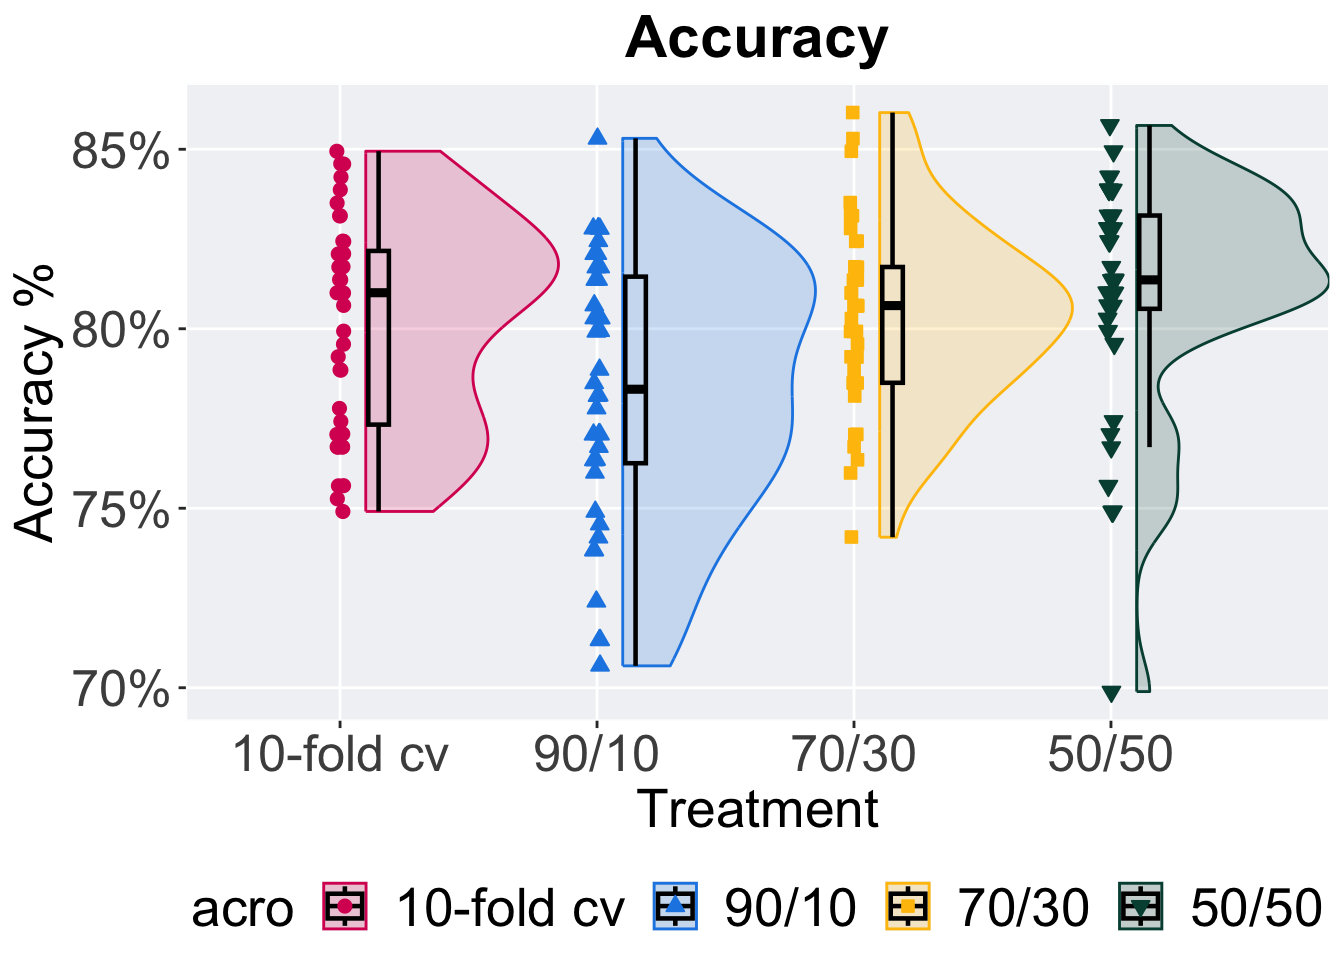
\includegraphics[width=1\linewidth]{lexidate-validation-supplemental_files/figure-latex/acc-task-3-plt-1}

Summary statistics for the generation a satisfactory solution is found.

\begin{Shaded}
\begin{Highlighting}[]
\NormalTok{performance }\OtherTok{\textless{}{-}} \FunctionTok{filter}\NormalTok{(scores, taskid }\SpecialCharTok{==}\NormalTok{ task\_id\_lists[}\DecValTok{3}\NormalTok{])}
\NormalTok{performance }\SpecialCharTok{\%\textgreater{}\%}
  \FunctionTok{group\_by}\NormalTok{(acro) }\SpecialCharTok{\%\textgreater{}\%}
\NormalTok{  dplyr}\SpecialCharTok{::}\FunctionTok{summarise}\NormalTok{(}
    \AttributeTok{count =} \FunctionTok{n}\NormalTok{(),}
    \AttributeTok{na\_cnt =} \FunctionTok{sum}\NormalTok{(}\FunctionTok{is.na}\NormalTok{(accuracy)),}
    \AttributeTok{min =} \FunctionTok{min}\NormalTok{(accuracy, }\AttributeTok{na.rm =} \ConstantTok{TRUE}\NormalTok{),}
    \AttributeTok{median =} \FunctionTok{median}\NormalTok{(accuracy, }\AttributeTok{na.rm =} \ConstantTok{TRUE}\NormalTok{),}
    \AttributeTok{mean =} \FunctionTok{mean}\NormalTok{(accuracy, }\AttributeTok{na.rm =} \ConstantTok{TRUE}\NormalTok{),}
    \AttributeTok{max =} \FunctionTok{max}\NormalTok{(accuracy, }\AttributeTok{na.rm =} \ConstantTok{TRUE}\NormalTok{),}
    \AttributeTok{IQR =} \FunctionTok{IQR}\NormalTok{(accuracy, }\AttributeTok{na.rm =} \ConstantTok{TRUE}\NormalTok{)}
\NormalTok{  )}
\end{Highlighting}
\end{Shaded}

\begin{verbatim}
## # A tibble: 4 x 8
##   acro       count na_cnt   min median  mean   max    IQR
##   <fct>      <int>  <int> <dbl>  <dbl> <dbl> <dbl>  <dbl>
## 1 10-fold cv    40      0 0.749  0.810 0.803 0.849 0.0484
## 2 90/10         40      0 0.706  0.783 0.783 0.853 0.0520
## 3 70/30         40      0 0.742  0.806 0.803 0.860 0.0323
## 4 50/50         40      0 0.699  0.814 0.811 0.857 0.0260
\end{verbatim}

Kruskal--Wallis test illustrates evidence of statistical differences.

\begin{Shaded}
\begin{Highlighting}[]
\FunctionTok{kruskal.test}\NormalTok{(accuracy }\SpecialCharTok{\textasciitilde{}}\NormalTok{ acro, }\AttributeTok{data =}\NormalTok{ performance)}
\end{Highlighting}
\end{Shaded}

\begin{verbatim}
## 
##  Kruskal-Wallis rank sum test
## 
## data:  accuracy by acro
## Kruskal-Wallis chi-squared = 14.599, df = 3, p-value = 0.002193
\end{verbatim}

Results for post-hoc Wilcoxon rank-sum test with a Bonferroni correction.

\begin{Shaded}
\begin{Highlighting}[]
\FunctionTok{pairwise.wilcox.test}\NormalTok{(}\AttributeTok{x =}\NormalTok{ performance}\SpecialCharTok{$}\NormalTok{accuracy, }\AttributeTok{g =}\NormalTok{ performance}\SpecialCharTok{$}\NormalTok{acro,}
                     \AttributeTok{p.adjust.method =} \StringTok{"bonferroni"}\NormalTok{,}
                     \AttributeTok{paired =} \ConstantTok{FALSE}\NormalTok{, }\AttributeTok{conf.int =} \ConstantTok{FALSE}\NormalTok{, }\AttributeTok{alternative =} \StringTok{"t"}\NormalTok{)}
\end{Highlighting}
\end{Shaded}

\begin{verbatim}
## 
##  Pairwise comparisons using Wilcoxon rank sum test with continuity correction 
## 
## data:  performance$accuracy and performance$acro 
## 
##       10-fold cv 90/10  70/30 
## 90/10 0.1097     -      -     
## 70/30 1.0000     0.1185 -     
## 50/50 1.0000     0.0026 0.2697
## 
## P value adjustment method: bonferroni
\end{verbatim}

\hypertarget{task-167161}{%
\subsection{Task 167161}\label{task-167161}}

\begin{Shaded}
\begin{Highlighting}[]
\FunctionTok{filter}\NormalTok{(scores, taskid }\SpecialCharTok{==}\NormalTok{ task\_id\_lists[}\DecValTok{4}\NormalTok{]) }\SpecialCharTok{\%\textgreater{}\%}
  \FunctionTok{ggplot}\NormalTok{(., }\FunctionTok{aes}\NormalTok{(}\AttributeTok{x =}\NormalTok{ acro, }\AttributeTok{y =}\NormalTok{ accuracy, }\AttributeTok{color =}\NormalTok{ acro,}
                \AttributeTok{fill =}\NormalTok{ acro, }\AttributeTok{shape =}\NormalTok{ acro)) }\SpecialCharTok{+}
  \FunctionTok{geom\_flat\_violin}\NormalTok{(}\AttributeTok{position =} \FunctionTok{position\_nudge}\NormalTok{(}\AttributeTok{x =} \FloatTok{0.1}\NormalTok{, }\AttributeTok{y =} \DecValTok{0}\NormalTok{),}
                   \AttributeTok{scale =} \StringTok{"width"}\NormalTok{, }\AttributeTok{alpha =} \FloatTok{0.2}\NormalTok{, }\AttributeTok{width =} \FloatTok{1.5}\NormalTok{) }\SpecialCharTok{+}
  \FunctionTok{geom\_boxplot}\NormalTok{(}\AttributeTok{color =} \StringTok{"black"}\NormalTok{, }\AttributeTok{width =}\NormalTok{ .}\DecValTok{08}\NormalTok{, }\AttributeTok{outlier.shape =} \ConstantTok{NA}\NormalTok{, }\AttributeTok{alpha =} \FloatTok{0.0}\NormalTok{,}
               \AttributeTok{size =} \FloatTok{0.8}\NormalTok{, }\AttributeTok{position =} \FunctionTok{position\_nudge}\NormalTok{(}\AttributeTok{x =}\NormalTok{ .}\DecValTok{15}\NormalTok{, }\AttributeTok{y =} \DecValTok{0}\NormalTok{)) }\SpecialCharTok{+}
  \FunctionTok{geom\_point}\NormalTok{(}\AttributeTok{position =} \FunctionTok{position\_jitter}\NormalTok{(}\AttributeTok{width =}\NormalTok{ .}\DecValTok{015}\NormalTok{, }\AttributeTok{height =}\NormalTok{ .}\DecValTok{0001}\NormalTok{),}
             \AttributeTok{size =} \FloatTok{2.0}\NormalTok{, }\AttributeTok{alpha =} \FloatTok{1.0}\NormalTok{) }\SpecialCharTok{+}
  \FunctionTok{scale\_y\_continuous}\NormalTok{(}
    \AttributeTok{name =} \StringTok{"Accuracy \%"}\NormalTok{,}
    \AttributeTok{limits=}\FunctionTok{c}\NormalTok{(.}\DecValTok{55}\NormalTok{, .}\DecValTok{80}\NormalTok{),}
    \AttributeTok{breaks=}\FunctionTok{c}\NormalTok{(.}\DecValTok{56}\NormalTok{,.}\DecValTok{64}\NormalTok{,.}\DecValTok{72}\NormalTok{,.}\DecValTok{8}\NormalTok{),}
    \AttributeTok{labels =}\NormalTok{ scales}\SpecialCharTok{::}\NormalTok{percent}

\NormalTok{  ) }\SpecialCharTok{+}
  \FunctionTok{scale\_x\_discrete}\NormalTok{(}
    \AttributeTok{name =} \StringTok{"Treatment"}
\NormalTok{  ) }\SpecialCharTok{+}
  \FunctionTok{scale\_shape\_manual}\NormalTok{(}\AttributeTok{values =}\NormalTok{ SHAPE) }\SpecialCharTok{+}
  \FunctionTok{scale\_colour\_manual}\NormalTok{(}\AttributeTok{values =}\NormalTok{ cb\_palette, ) }\SpecialCharTok{+}
  \FunctionTok{scale\_fill\_manual}\NormalTok{(}\AttributeTok{values =}\NormalTok{ cb\_palette) }\SpecialCharTok{+}
  \FunctionTok{ggtitle}\NormalTok{(}\StringTok{"Accuracy"}\NormalTok{) }\SpecialCharTok{+}
\NormalTok{  p\_theme }\SpecialCharTok{+}
  \FunctionTok{guides}\NormalTok{(}
    \AttributeTok{shape=}\FunctionTok{guide\_legend}\NormalTok{(}\AttributeTok{nrow =} \DecValTok{1}\NormalTok{, }\AttributeTok{title.position =} \StringTok{"bottom"}\NormalTok{,}
                       \AttributeTok{title =} \StringTok{"Evaluation strategy"}\NormalTok{),}
    \AttributeTok{color=}\FunctionTok{guide\_legend}\NormalTok{(}\AttributeTok{nrow =} \DecValTok{1}\NormalTok{, }\AttributeTok{title.position =} \StringTok{"bottom"}\NormalTok{,}
                       \AttributeTok{title =} \StringTok{"Evaluation strategy"}\NormalTok{),}
    \AttributeTok{fill=}\FunctionTok{guide\_legend}\NormalTok{(}\AttributeTok{nrow =} \DecValTok{1}\NormalTok{, }\AttributeTok{title.position =} \StringTok{"bottom"}\NormalTok{,}
                      \AttributeTok{title =} \StringTok{"Evaluation strategy"}\NormalTok{)}
\NormalTok{  )}
\end{Highlighting}
\end{Shaded}

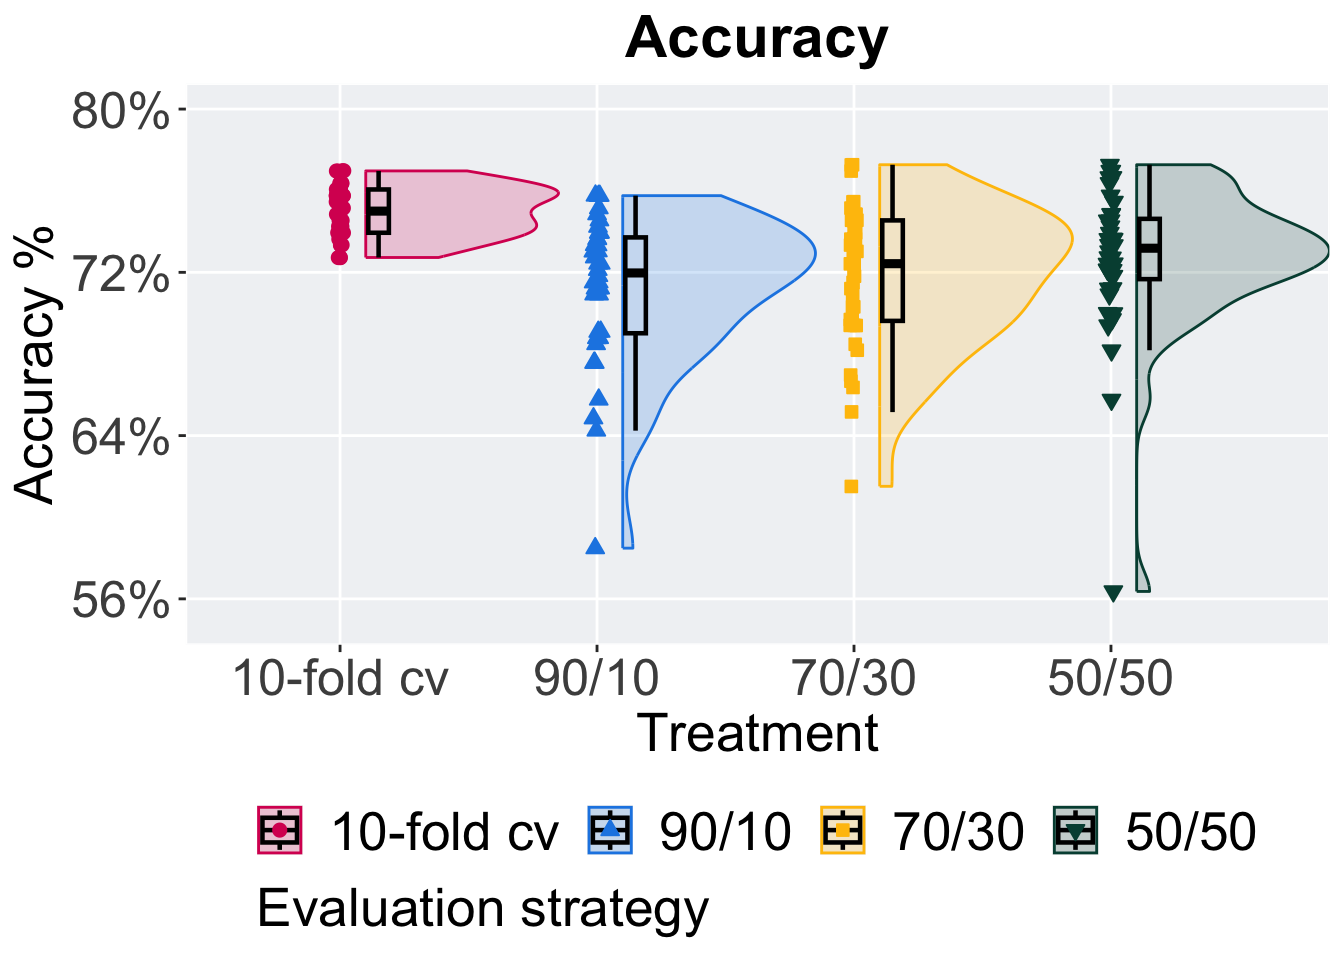
\includegraphics[width=1\linewidth]{lexidate-validation-supplemental_files/figure-latex/acc-task-4-plt-1}

Summary statistics for the generation a satisfactory solution is found.

\begin{Shaded}
\begin{Highlighting}[]
\NormalTok{performance }\OtherTok{\textless{}{-}} \FunctionTok{filter}\NormalTok{(scores, taskid }\SpecialCharTok{==}\NormalTok{ task\_id\_lists[}\DecValTok{4}\NormalTok{])}
\NormalTok{performance }\SpecialCharTok{\%\textgreater{}\%}
  \FunctionTok{group\_by}\NormalTok{(acro) }\SpecialCharTok{\%\textgreater{}\%}
\NormalTok{  dplyr}\SpecialCharTok{::}\FunctionTok{summarise}\NormalTok{(}
    \AttributeTok{count =} \FunctionTok{n}\NormalTok{(),}
    \AttributeTok{na\_cnt =} \FunctionTok{sum}\NormalTok{(}\FunctionTok{is.na}\NormalTok{(accuracy)),}
    \AttributeTok{min =} \FunctionTok{min}\NormalTok{(accuracy, }\AttributeTok{na.rm =} \ConstantTok{TRUE}\NormalTok{),}
    \AttributeTok{median =} \FunctionTok{median}\NormalTok{(accuracy, }\AttributeTok{na.rm =} \ConstantTok{TRUE}\NormalTok{),}
    \AttributeTok{mean =} \FunctionTok{mean}\NormalTok{(accuracy, }\AttributeTok{na.rm =} \ConstantTok{TRUE}\NormalTok{),}
    \AttributeTok{max =} \FunctionTok{max}\NormalTok{(accuracy, }\AttributeTok{na.rm =} \ConstantTok{TRUE}\NormalTok{),}
    \AttributeTok{IQR =} \FunctionTok{IQR}\NormalTok{(accuracy, }\AttributeTok{na.rm =} \ConstantTok{TRUE}\NormalTok{)}
\NormalTok{  )}
\end{Highlighting}
\end{Shaded}

\begin{verbatim}
## # A tibble: 4 x 8
##   acro       count na_cnt   min median  mean   max    IQR
##   <fct>      <int>  <int> <dbl>  <dbl> <dbl> <dbl>  <dbl>
## 1 10-fold cv    40      0 0.727  0.75  0.75  0.770 0.0212
## 2 90/10         40      0 0.585  0.720 0.712 0.758 0.0470
## 3 70/30         40      0 0.615  0.724 0.718 0.773 0.0492
## 4 50/50         40      0 0.564  0.732 0.727 0.773 0.0295
\end{verbatim}

Kruskal--Wallis test illustrates evidence of statistical differences.

\begin{Shaded}
\begin{Highlighting}[]
\FunctionTok{kruskal.test}\NormalTok{(accuracy }\SpecialCharTok{\textasciitilde{}}\NormalTok{ acro, }\AttributeTok{data =}\NormalTok{ performance)}
\end{Highlighting}
\end{Shaded}

\begin{verbatim}
## 
##  Kruskal-Wallis rank sum test
## 
## data:  accuracy by acro
## Kruskal-Wallis chi-squared = 37.759, df = 3, p-value = 3.179e-08
\end{verbatim}

Results for post-hoc Wilcoxon rank-sum test with a Bonferroni correction.

\begin{Shaded}
\begin{Highlighting}[]
\FunctionTok{pairwise.wilcox.test}\NormalTok{(}\AttributeTok{x =}\NormalTok{ performance}\SpecialCharTok{$}\NormalTok{accuracy, }\AttributeTok{g =}\NormalTok{ performance}\SpecialCharTok{$}\NormalTok{acro,}
                     \AttributeTok{p.adjust.method =} \StringTok{"bonferroni"}\NormalTok{,}
                     \AttributeTok{paired =} \ConstantTok{FALSE}\NormalTok{, }\AttributeTok{conf.int =} \ConstantTok{FALSE}\NormalTok{, }\AttributeTok{alternative =} \StringTok{"t"}\NormalTok{)}
\end{Highlighting}
\end{Shaded}

\begin{verbatim}
## 
##  Pairwise comparisons using Wilcoxon rank sum test with continuity correction 
## 
## data:  performance$accuracy and performance$acro 
## 
##       10-fold cv 90/10   70/30  
## 90/10 5.7e-08    -       -      
## 70/30 2.2e-05    1.00000 -      
## 50/50 0.00077    0.27098 1.00000
## 
## P value adjustment method: bonferroni
\end{verbatim}

\hypertarget{task-167185}{%
\subsection{Task 167185}\label{task-167185}}

\begin{Shaded}
\begin{Highlighting}[]
\FunctionTok{filter}\NormalTok{(scores, taskid }\SpecialCharTok{==}\NormalTok{ task\_id\_lists[}\DecValTok{5}\NormalTok{]) }\SpecialCharTok{\%\textgreater{}\%}
  \FunctionTok{ggplot}\NormalTok{(., }\FunctionTok{aes}\NormalTok{(}\AttributeTok{x =}\NormalTok{ acro, }\AttributeTok{y =}\NormalTok{ accuracy, }\AttributeTok{color =}\NormalTok{ acro,}
                \AttributeTok{fill =}\NormalTok{ acro, }\AttributeTok{shape =}\NormalTok{ acro)) }\SpecialCharTok{+}
  \FunctionTok{geom\_flat\_violin}\NormalTok{(}\AttributeTok{position =} \FunctionTok{position\_nudge}\NormalTok{(}\AttributeTok{x =} \FloatTok{0.1}\NormalTok{, }\AttributeTok{y =} \DecValTok{0}\NormalTok{),}
                   \AttributeTok{scale =} \StringTok{"width"}\NormalTok{, }\AttributeTok{alpha =} \FloatTok{0.2}\NormalTok{, }\AttributeTok{width =} \FloatTok{1.5}\NormalTok{) }\SpecialCharTok{+}
  \FunctionTok{geom\_boxplot}\NormalTok{(}\AttributeTok{color =} \StringTok{"black"}\NormalTok{, }\AttributeTok{width =}\NormalTok{ .}\DecValTok{08}\NormalTok{, }\AttributeTok{outlier.shape =} \ConstantTok{NA}\NormalTok{, }\AttributeTok{alpha =} \FloatTok{0.0}\NormalTok{,}
               \AttributeTok{size =} \FloatTok{0.8}\NormalTok{, }\AttributeTok{position =} \FunctionTok{position\_nudge}\NormalTok{(}\AttributeTok{x =}\NormalTok{ .}\DecValTok{15}\NormalTok{, }\AttributeTok{y =} \DecValTok{0}\NormalTok{)) }\SpecialCharTok{+}
  \FunctionTok{geom\_point}\NormalTok{(}\AttributeTok{position =} \FunctionTok{position\_jitter}\NormalTok{(}\AttributeTok{width =}\NormalTok{ .}\DecValTok{015}\NormalTok{, }\AttributeTok{height =}\NormalTok{ .}\DecValTok{0001}\NormalTok{),}
             \AttributeTok{size =} \FloatTok{2.0}\NormalTok{, }\AttributeTok{alpha =} \FloatTok{1.0}\NormalTok{) }\SpecialCharTok{+}
  \FunctionTok{scale\_y\_continuous}\NormalTok{(}
    \AttributeTok{name =} \StringTok{"Accuracy \%"}\NormalTok{,}
    \AttributeTok{limits=}\FunctionTok{c}\NormalTok{(.}\DecValTok{86}\NormalTok{, .}\DecValTok{96}\NormalTok{),}
    \AttributeTok{breaks=}\FunctionTok{c}\NormalTok{(.}\DecValTok{86}\NormalTok{,.}\DecValTok{91}\NormalTok{,.}\DecValTok{96}\NormalTok{),}
    \AttributeTok{labels =}\NormalTok{ scales}\SpecialCharTok{::}\NormalTok{percent}

\NormalTok{  ) }\SpecialCharTok{+}
  \FunctionTok{scale\_x\_discrete}\NormalTok{(}
    \AttributeTok{name =} \StringTok{"Treatment"}
\NormalTok{  ) }\SpecialCharTok{+}
  \FunctionTok{scale\_shape\_manual}\NormalTok{(}\AttributeTok{values =}\NormalTok{ SHAPE) }\SpecialCharTok{+}
  \FunctionTok{scale\_colour\_manual}\NormalTok{(}\AttributeTok{values =}\NormalTok{ cb\_palette, ) }\SpecialCharTok{+}
  \FunctionTok{scale\_fill\_manual}\NormalTok{(}\AttributeTok{values =}\NormalTok{ cb\_palette) }\SpecialCharTok{+}
  \FunctionTok{ggtitle}\NormalTok{(}\StringTok{"Accuracy"}\NormalTok{) }\SpecialCharTok{+}
\NormalTok{  p\_theme }\SpecialCharTok{+}
  \FunctionTok{guides}\NormalTok{(}
    \AttributeTok{shape=}\FunctionTok{guide\_legend}\NormalTok{(}\AttributeTok{nrow =} \DecValTok{1}\NormalTok{, }\AttributeTok{title.position =} \StringTok{"bottom"}\NormalTok{,}
                       \AttributeTok{title =} \StringTok{"Evaluation strategy"}\NormalTok{),}
    \AttributeTok{color=}\FunctionTok{guide\_legend}\NormalTok{(}\AttributeTok{nrow =} \DecValTok{1}\NormalTok{, }\AttributeTok{title.position =} \StringTok{"bottom"}\NormalTok{,}
                       \AttributeTok{title =} \StringTok{"Evaluation strategy"}\NormalTok{),}
    \AttributeTok{fill=}\FunctionTok{guide\_legend}\NormalTok{(}\AttributeTok{nrow =} \DecValTok{1}\NormalTok{, }\AttributeTok{title.position =} \StringTok{"bottom"}\NormalTok{,}
                      \AttributeTok{title =} \StringTok{"Evaluation strategy"}\NormalTok{)}
\NormalTok{  )}
\end{Highlighting}
\end{Shaded}

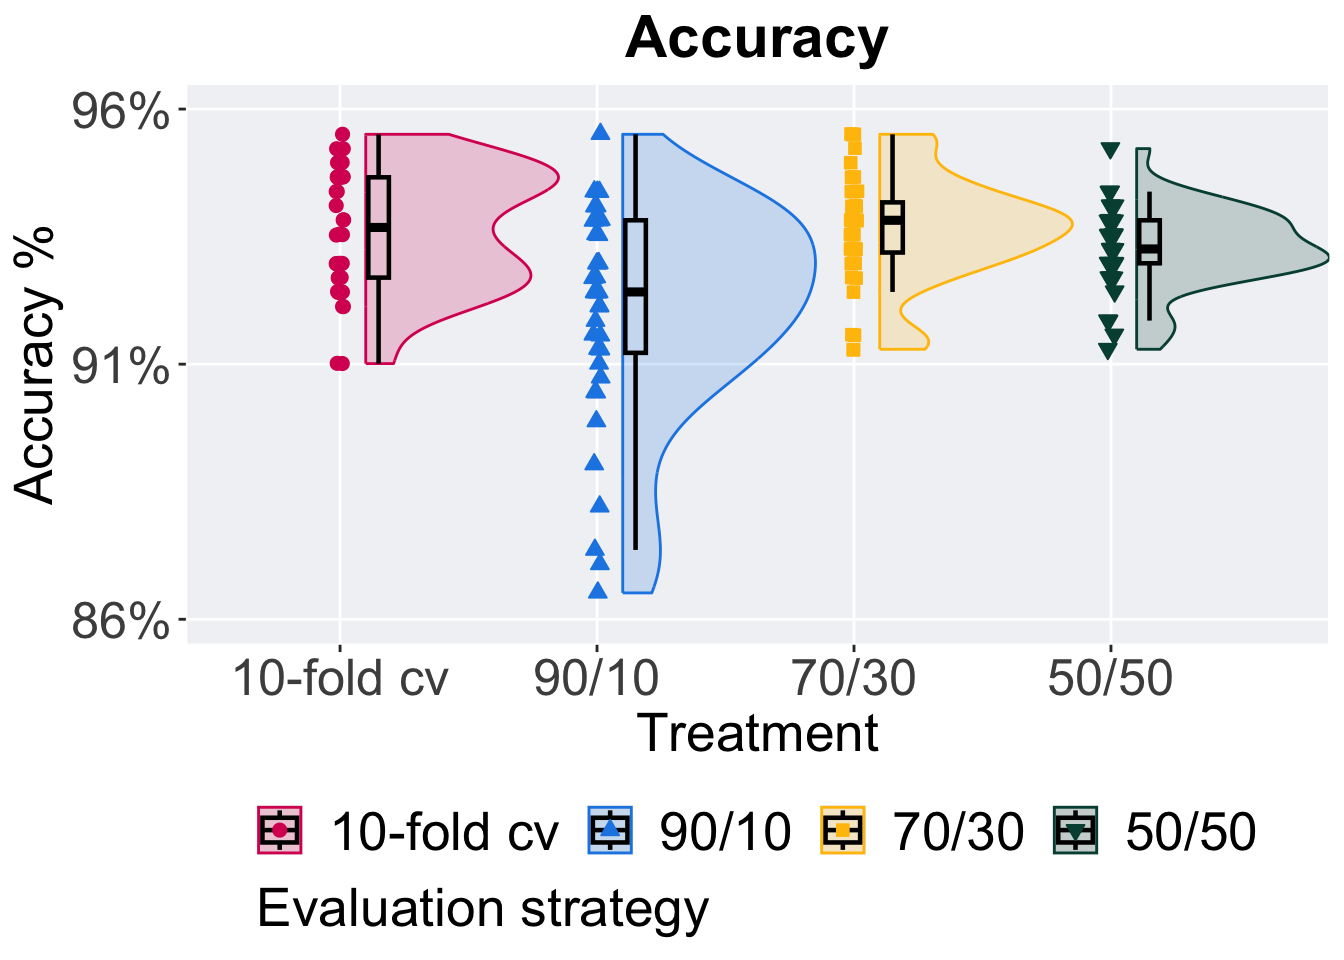
\includegraphics[width=1\linewidth]{lexidate-validation-supplemental_files/figure-latex/acc-task-5-plt-1}

Summary statistics for the generation a satisfactory solution is found.

\begin{Shaded}
\begin{Highlighting}[]
\NormalTok{performance }\OtherTok{\textless{}{-}} \FunctionTok{filter}\NormalTok{(scores, taskid }\SpecialCharTok{==}\NormalTok{ task\_id\_lists[}\DecValTok{5}\NormalTok{])}
\NormalTok{performance }\SpecialCharTok{\%\textgreater{}\%}
  \FunctionTok{group\_by}\NormalTok{(acro) }\SpecialCharTok{\%\textgreater{}\%}
\NormalTok{  dplyr}\SpecialCharTok{::}\FunctionTok{summarise}\NormalTok{(}
    \AttributeTok{count =} \FunctionTok{n}\NormalTok{(),}
    \AttributeTok{na\_cnt =} \FunctionTok{sum}\NormalTok{(}\FunctionTok{is.na}\NormalTok{(accuracy)),}
    \AttributeTok{min =} \FunctionTok{min}\NormalTok{(accuracy, }\AttributeTok{na.rm =} \ConstantTok{TRUE}\NormalTok{),}
    \AttributeTok{median =} \FunctionTok{median}\NormalTok{(accuracy, }\AttributeTok{na.rm =} \ConstantTok{TRUE}\NormalTok{),}
    \AttributeTok{mean =} \FunctionTok{mean}\NormalTok{(accuracy, }\AttributeTok{na.rm =} \ConstantTok{TRUE}\NormalTok{),}
    \AttributeTok{max =} \FunctionTok{max}\NormalTok{(accuracy, }\AttributeTok{na.rm =} \ConstantTok{TRUE}\NormalTok{),}
    \AttributeTok{IQR =} \FunctionTok{IQR}\NormalTok{(accuracy, }\AttributeTok{na.rm =} \ConstantTok{TRUE}\NormalTok{)}
\NormalTok{  )}
\end{Highlighting}
\end{Shaded}

\begin{verbatim}
## # A tibble: 4 x 8
##   acro       count na_cnt   min median  mean   max     IQR
##   <fct>      <int>  <int> <dbl>  <dbl> <dbl> <dbl>   <dbl>
## 1 10-fold cv    40      0 0.910  0.937 0.936 0.955 0.0197 
## 2 90/10         40      0 0.865  0.924 0.920 0.955 0.0260 
## 3 70/30         40      0 0.913  0.938 0.936 0.955 0.00983
## 4 50/50         40      0 0.913  0.933 0.933 0.952 0.00843
\end{verbatim}

Kruskal--Wallis test illustrates evidence of statistical differences.

\begin{Shaded}
\begin{Highlighting}[]
\FunctionTok{kruskal.test}\NormalTok{(accuracy }\SpecialCharTok{\textasciitilde{}}\NormalTok{ acro, }\AttributeTok{data =}\NormalTok{ performance)}
\end{Highlighting}
\end{Shaded}

\begin{verbatim}
## 
##  Kruskal-Wallis rank sum test
## 
## data:  accuracy by acro
## Kruskal-Wallis chi-squared = 20.962, df = 3, p-value = 0.0001072
\end{verbatim}

Results for post-hoc Wilcoxon rank-sum test with a Bonferroni correction.

\begin{Shaded}
\begin{Highlighting}[]
\FunctionTok{pairwise.wilcox.test}\NormalTok{(}\AttributeTok{x =}\NormalTok{ performance}\SpecialCharTok{$}\NormalTok{accuracy, }\AttributeTok{g =}\NormalTok{ performance}\SpecialCharTok{$}\NormalTok{acro,}
                     \AttributeTok{p.adjust.method =} \StringTok{"bonferroni"}\NormalTok{,}
                     \AttributeTok{paired =} \ConstantTok{FALSE}\NormalTok{, }\AttributeTok{conf.int =} \ConstantTok{FALSE}\NormalTok{, }\AttributeTok{alternative =} \StringTok{"t"}\NormalTok{)}
\end{Highlighting}
\end{Shaded}

\begin{verbatim}
## 
##  Pairwise comparisons using Wilcoxon rank sum test with continuity correction 
## 
## data:  performance$accuracy and performance$acro 
## 
##       10-fold cv 90/10   70/30  
## 90/10 0.00095    -       -      
## 70/30 1.00000    0.00110 -      
## 50/50 0.89845    0.03149 0.30642
## 
## P value adjustment method: bonferroni
\end{verbatim}

\hypertarget{task-189905}{%
\subsection{Task 189905}\label{task-189905}}

\begin{Shaded}
\begin{Highlighting}[]
\FunctionTok{filter}\NormalTok{(scores, taskid }\SpecialCharTok{==}\NormalTok{ task\_id\_lists[}\DecValTok{6}\NormalTok{]) }\SpecialCharTok{\%\textgreater{}\%}
  \FunctionTok{ggplot}\NormalTok{(., }\FunctionTok{aes}\NormalTok{(}\AttributeTok{x =}\NormalTok{ acro, }\AttributeTok{y =}\NormalTok{ accuracy, }\AttributeTok{color =}\NormalTok{ acro,}
                \AttributeTok{fill =}\NormalTok{ acro, }\AttributeTok{shape =}\NormalTok{ acro)) }\SpecialCharTok{+}
  \FunctionTok{geom\_flat\_violin}\NormalTok{(}\AttributeTok{position =} \FunctionTok{position\_nudge}\NormalTok{(}\AttributeTok{x =} \FloatTok{0.1}\NormalTok{, }\AttributeTok{y =} \DecValTok{0}\NormalTok{),}
                   \AttributeTok{scale =} \StringTok{"width"}\NormalTok{, }\AttributeTok{alpha =} \FloatTok{0.2}\NormalTok{, }\AttributeTok{width =} \FloatTok{1.5}\NormalTok{) }\SpecialCharTok{+}
  \FunctionTok{geom\_boxplot}\NormalTok{(}\AttributeTok{color =} \StringTok{"black"}\NormalTok{, }\AttributeTok{width =}\NormalTok{ .}\DecValTok{08}\NormalTok{, }\AttributeTok{outlier.shape =} \ConstantTok{NA}\NormalTok{, }\AttributeTok{alpha =} \FloatTok{0.0}\NormalTok{,}
               \AttributeTok{size =} \FloatTok{0.8}\NormalTok{, }\AttributeTok{position =} \FunctionTok{position\_nudge}\NormalTok{(}\AttributeTok{x =}\NormalTok{ .}\DecValTok{15}\NormalTok{, }\AttributeTok{y =} \DecValTok{0}\NormalTok{)) }\SpecialCharTok{+}
  \FunctionTok{geom\_point}\NormalTok{(}\AttributeTok{position =} \FunctionTok{position\_jitter}\NormalTok{(}\AttributeTok{width =}\NormalTok{ .}\DecValTok{015}\NormalTok{, }\AttributeTok{height =}\NormalTok{ .}\DecValTok{0001}\NormalTok{),}
             \AttributeTok{size =} \FloatTok{2.0}\NormalTok{, }\AttributeTok{alpha =} \FloatTok{1.0}\NormalTok{) }\SpecialCharTok{+}
  \FunctionTok{scale\_y\_continuous}\NormalTok{(}
    \AttributeTok{name =} \StringTok{"Accuracy \%"}\NormalTok{,}
    \AttributeTok{limits=}\FunctionTok{c}\NormalTok{(.}\DecValTok{916}\NormalTok{,}\FloatTok{1.001}\NormalTok{),}
    \AttributeTok{breaks=}\FunctionTok{c}\NormalTok{(.}\DecValTok{92}\NormalTok{,.}\DecValTok{96}\NormalTok{,}\DecValTok{1}\NormalTok{),}
    \AttributeTok{labels =}\NormalTok{ scales}\SpecialCharTok{::}\NormalTok{percent}

\NormalTok{  ) }\SpecialCharTok{+}
  \FunctionTok{scale\_x\_discrete}\NormalTok{(}
    \AttributeTok{name =} \StringTok{"Treatment"}
\NormalTok{  ) }\SpecialCharTok{+}
  \FunctionTok{scale\_shape\_manual}\NormalTok{(}\AttributeTok{values =}\NormalTok{ SHAPE) }\SpecialCharTok{+}
  \FunctionTok{scale\_colour\_manual}\NormalTok{(}\AttributeTok{values =}\NormalTok{ cb\_palette, ) }\SpecialCharTok{+}
  \FunctionTok{scale\_fill\_manual}\NormalTok{(}\AttributeTok{values =}\NormalTok{ cb\_palette) }\SpecialCharTok{+}
  \FunctionTok{ggtitle}\NormalTok{(}\StringTok{"Accuracy"}\NormalTok{) }\SpecialCharTok{+}
\NormalTok{  p\_theme }\SpecialCharTok{+}
  \FunctionTok{guides}\NormalTok{(}
    \AttributeTok{shape=}\FunctionTok{guide\_legend}\NormalTok{(}\AttributeTok{nrow =} \DecValTok{1}\NormalTok{, }\AttributeTok{title.position =} \StringTok{"bottom"}\NormalTok{,}
                       \AttributeTok{title =} \StringTok{"Evaluation strategy"}\NormalTok{),}
    \AttributeTok{color=}\FunctionTok{guide\_legend}\NormalTok{(}\AttributeTok{nrow =} \DecValTok{1}\NormalTok{, }\AttributeTok{title.position =} \StringTok{"bottom"}\NormalTok{,}
                       \AttributeTok{title =} \StringTok{"Evaluation strategy"}\NormalTok{),}
    \AttributeTok{fill=}\FunctionTok{guide\_legend}\NormalTok{(}\AttributeTok{nrow =} \DecValTok{1}\NormalTok{, }\AttributeTok{title.position =} \StringTok{"bottom"}\NormalTok{,}
                      \AttributeTok{title =} \StringTok{"Evaluation strategy"}\NormalTok{)}
\NormalTok{  )}
\end{Highlighting}
\end{Shaded}

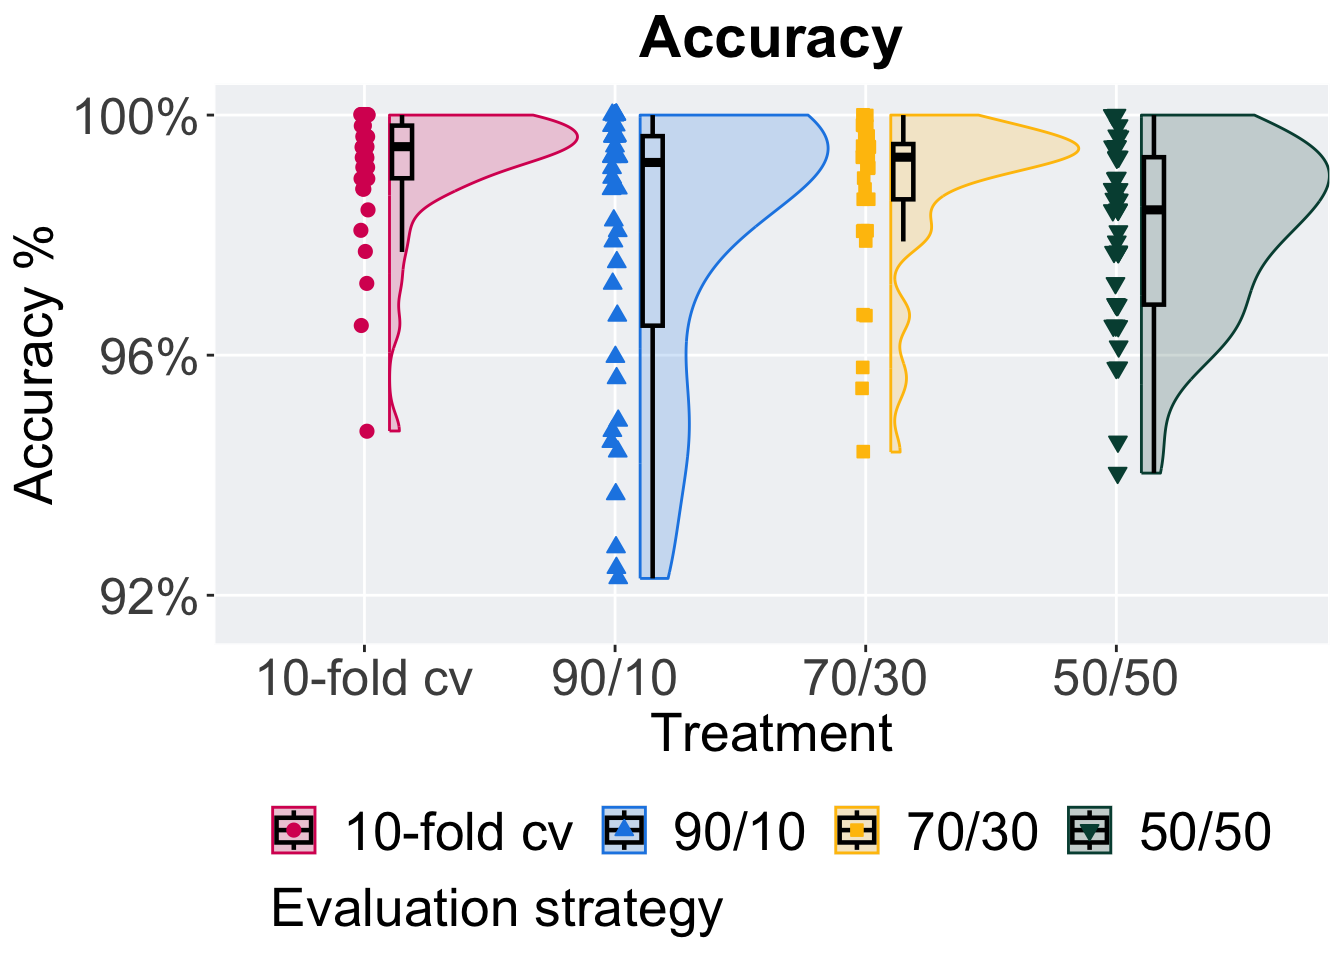
\includegraphics[width=1\linewidth]{lexidate-validation-supplemental_files/figure-latex/acc-task-6-plt-1}

Summary statistics for the generation a satisfactory solution is found.

\begin{Shaded}
\begin{Highlighting}[]
\NormalTok{performance }\OtherTok{\textless{}{-}} \FunctionTok{filter}\NormalTok{(scores, taskid }\SpecialCharTok{==}\NormalTok{ task\_id\_lists[}\DecValTok{6}\NormalTok{])}
\NormalTok{performance }\SpecialCharTok{\%\textgreater{}\%}
  \FunctionTok{group\_by}\NormalTok{(acro) }\SpecialCharTok{\%\textgreater{}\%}
\NormalTok{  dplyr}\SpecialCharTok{::}\FunctionTok{summarise}\NormalTok{(}
    \AttributeTok{count =} \FunctionTok{n}\NormalTok{(),}
    \AttributeTok{na\_cnt =} \FunctionTok{sum}\NormalTok{(}\FunctionTok{is.na}\NormalTok{(accuracy)),}
    \AttributeTok{min =} \FunctionTok{min}\NormalTok{(accuracy, }\AttributeTok{na.rm =} \ConstantTok{TRUE}\NormalTok{),}
    \AttributeTok{median =} \FunctionTok{median}\NormalTok{(accuracy, }\AttributeTok{na.rm =} \ConstantTok{TRUE}\NormalTok{),}
    \AttributeTok{mean =} \FunctionTok{mean}\NormalTok{(accuracy, }\AttributeTok{na.rm =} \ConstantTok{TRUE}\NormalTok{),}
    \AttributeTok{max =} \FunctionTok{max}\NormalTok{(accuracy, }\AttributeTok{na.rm =} \ConstantTok{TRUE}\NormalTok{),}
    \AttributeTok{IQR =} \FunctionTok{IQR}\NormalTok{(accuracy, }\AttributeTok{na.rm =} \ConstantTok{TRUE}\NormalTok{)}
\NormalTok{  )}
\end{Highlighting}
\end{Shaded}

\begin{verbatim}
## # A tibble: 4 x 8
##   acro       count na_cnt   min median  mean   max     IQR
##   <fct>      <int>  <int> <dbl>  <dbl> <dbl> <dbl>   <dbl>
## 1 10-fold cv    40      0 0.947  0.995 0.992     1 0.00877
## 2 90/10         40      0 0.923  0.992 0.979     1 0.0316 
## 3 70/30         40      0 0.944  0.993 0.988     1 0.00921
## 4 50/50         40      0 0.940  0.984 0.980     1 0.0246
\end{verbatim}

Kruskal--Wallis test illustrates evidence of statistical differences.

\begin{Shaded}
\begin{Highlighting}[]
\FunctionTok{kruskal.test}\NormalTok{(accuracy }\SpecialCharTok{\textasciitilde{}}\NormalTok{ acro, }\AttributeTok{data =}\NormalTok{ performance)}
\end{Highlighting}
\end{Shaded}

\begin{verbatim}
## 
##  Kruskal-Wallis rank sum test
## 
## data:  accuracy by acro
## Kruskal-Wallis chi-squared = 15.64, df = 3, p-value = 0.001344
\end{verbatim}

Results for post-hoc Wilcoxon rank-sum test with a Bonferroni correction.

\begin{Shaded}
\begin{Highlighting}[]
\FunctionTok{pairwise.wilcox.test}\NormalTok{(}\AttributeTok{x =}\NormalTok{ performance}\SpecialCharTok{$}\NormalTok{accuracy, }\AttributeTok{g =}\NormalTok{ performance}\SpecialCharTok{$}\NormalTok{acro,}
                     \AttributeTok{p.adjust.method =} \StringTok{"bonferroni"}\NormalTok{,}
                     \AttributeTok{paired =} \ConstantTok{FALSE}\NormalTok{, }\AttributeTok{conf.int =} \ConstantTok{FALSE}\NormalTok{, }\AttributeTok{alternative =} \StringTok{"t"}\NormalTok{)}
\end{Highlighting}
\end{Shaded}

\begin{verbatim}
## 
##  Pairwise comparisons using Wilcoxon rank sum test with continuity correction 
## 
## data:  performance$accuracy and performance$acro 
## 
##       10-fold cv 90/10   70/30  
## 90/10 0.25039    -       -      
## 70/30 0.72764    1.00000 -      
## 50/50 0.00044    1.00000 0.03839
## 
## P value adjustment method: bonferroni
\end{verbatim}

\hypertarget{complexity-results}{%
\chapter{Complexity results}\label{complexity-results}}

Here we report the complexity for \textbf{final pipeline returned from a TPOT2 run} on each OpenML task.
40 replicates were conducted for each evaluation strategy explored.

\hypertarget{analysis-setup-1}{%
\section{Analysis setup}\label{analysis-setup-1}}

\begin{Shaded}
\begin{Highlighting}[]
\FunctionTok{library}\NormalTok{(ggplot2)}
\FunctionTok{library}\NormalTok{(cowplot)}
\FunctionTok{library}\NormalTok{(dplyr)}
\FunctionTok{library}\NormalTok{(PupillometryR)}

\NormalTok{comps }\OtherTok{\textless{}{-}} \FunctionTok{read.csv}\NormalTok{(}\StringTok{"./complexity.csv"}\NormalTok{, }\AttributeTok{header =} \ConstantTok{TRUE}\NormalTok{, }\AttributeTok{stringsAsFactors =} \ConstantTok{FALSE}\NormalTok{)}
\NormalTok{comps}\SpecialCharTok{$}\NormalTok{acro }\OtherTok{\textless{}{-}} \FunctionTok{factor}\NormalTok{(comps}\SpecialCharTok{$}\NormalTok{acro, }\AttributeTok{levels =}\NormalTok{ NAMES)}
\end{Highlighting}
\end{Shaded}

\hypertarget{accuracy-per-openml-task-1}{%
\section{Accuracy per OpenML task}\label{accuracy-per-openml-task-1}}

Accuracy of the returned pipeline from an evolutionary run.

\hypertarget{task-167104-1}{%
\subsection{Task 167104}\label{task-167104-1}}

\begin{Shaded}
\begin{Highlighting}[]
\FunctionTok{filter}\NormalTok{(comps, taskid }\SpecialCharTok{==}\NormalTok{ task\_id\_lists[}\DecValTok{1}\NormalTok{]) }\SpecialCharTok{\%\textgreater{}\%}
  \FunctionTok{ggplot}\NormalTok{(., }\FunctionTok{aes}\NormalTok{(}\AttributeTok{x =}\NormalTok{ acro, }\AttributeTok{y =}\NormalTok{ complexity, }\AttributeTok{color =}\NormalTok{ acro,}
                \AttributeTok{fill =}\NormalTok{ acro, }\AttributeTok{shape =}\NormalTok{ acro)) }\SpecialCharTok{+}
  \FunctionTok{geom\_flat\_violin}\NormalTok{(}\AttributeTok{position =} \FunctionTok{position\_nudge}\NormalTok{(}\AttributeTok{x =} \FloatTok{0.1}\NormalTok{, }\AttributeTok{y =} \DecValTok{0}\NormalTok{),}
                   \AttributeTok{scale =} \StringTok{"width"}\NormalTok{, }\AttributeTok{alpha =} \FloatTok{0.2}\NormalTok{, }\AttributeTok{width =} \FloatTok{1.5}\NormalTok{) }\SpecialCharTok{+}
  \FunctionTok{geom\_boxplot}\NormalTok{(}\AttributeTok{color =} \StringTok{"black"}\NormalTok{, }\AttributeTok{width =}\NormalTok{ .}\DecValTok{08}\NormalTok{, }\AttributeTok{outlier.shape =} \ConstantTok{NA}\NormalTok{, }\AttributeTok{alpha =} \FloatTok{0.0}\NormalTok{,}
               \AttributeTok{size =} \FloatTok{0.8}\NormalTok{, }\AttributeTok{position =} \FunctionTok{position\_nudge}\NormalTok{(}\AttributeTok{x =}\NormalTok{ .}\DecValTok{15}\NormalTok{, }\AttributeTok{y =} \DecValTok{0}\NormalTok{)) }\SpecialCharTok{+}
  \FunctionTok{geom\_point}\NormalTok{(}\AttributeTok{position =} \FunctionTok{position\_jitter}\NormalTok{(}\AttributeTok{width =}\NormalTok{ .}\DecValTok{015}\NormalTok{, }\AttributeTok{height =}\NormalTok{ .}\DecValTok{0001}\NormalTok{),}
             \AttributeTok{size =} \FloatTok{2.0}\NormalTok{, }\AttributeTok{alpha =} \FloatTok{1.0}\NormalTok{) }\SpecialCharTok{+}
  \FunctionTok{scale\_y\_log10}\NormalTok{(}
    \AttributeTok{name =} \StringTok{"Complexity"}\NormalTok{,}
    \AttributeTok{breaks =} \FunctionTok{trans\_breaks}\NormalTok{(}\StringTok{"log10"}\NormalTok{, }\ControlFlowTok{function}\NormalTok{(x) }\DecValTok{10}\SpecialCharTok{\^{}}\NormalTok{x),}
    \AttributeTok{labels =} \FunctionTok{trans\_format}\NormalTok{(}\StringTok{"log10"}\NormalTok{, }\FunctionTok{math\_format}\NormalTok{(}\DecValTok{10}\SpecialCharTok{\^{}}\NormalTok{.x))}
\NormalTok{  ) }\SpecialCharTok{+}
  \FunctionTok{scale\_x\_discrete}\NormalTok{(}
    \AttributeTok{name =} \StringTok{"Treatment"}
\NormalTok{  ) }\SpecialCharTok{+}
  \FunctionTok{scale\_shape\_manual}\NormalTok{(}\AttributeTok{values =}\NormalTok{ SHAPE,) }\SpecialCharTok{+}
  \FunctionTok{scale\_colour\_manual}\NormalTok{(}\AttributeTok{values =}\NormalTok{ cb\_palette,) }\SpecialCharTok{+}
  \FunctionTok{scale\_fill\_manual}\NormalTok{(}\AttributeTok{values =}\NormalTok{ cb\_palette,) }\SpecialCharTok{+}
  \FunctionTok{ggtitle}\NormalTok{(}\StringTok{"Complexity"}\NormalTok{) }\SpecialCharTok{+}
\NormalTok{  p\_theme }\SpecialCharTok{+}
  \FunctionTok{guides}\NormalTok{(}
    \AttributeTok{shape=}\FunctionTok{guide\_legend}\NormalTok{(}\AttributeTok{nrow =} \DecValTok{1}\NormalTok{, }\AttributeTok{title.position =} \StringTok{"bottom"}\NormalTok{,}
                       \AttributeTok{title =} \StringTok{"Evaluation strategy"}\NormalTok{),}
    \AttributeTok{color=}\FunctionTok{guide\_legend}\NormalTok{(}\AttributeTok{nrow =} \DecValTok{1}\NormalTok{, }\AttributeTok{title.position =} \StringTok{"bottom"}\NormalTok{,}
                       \AttributeTok{title =} \StringTok{"Evaluation strategy"}\NormalTok{),}
    \AttributeTok{fill=}\FunctionTok{guide\_legend}\NormalTok{(}\AttributeTok{nrow =} \DecValTok{1}\NormalTok{, }\AttributeTok{title.position =} \StringTok{"bottom"}\NormalTok{,}
                      \AttributeTok{title =} \StringTok{"Evaluation strategy"}\NormalTok{)}
\NormalTok{  )}
\end{Highlighting}
\end{Shaded}

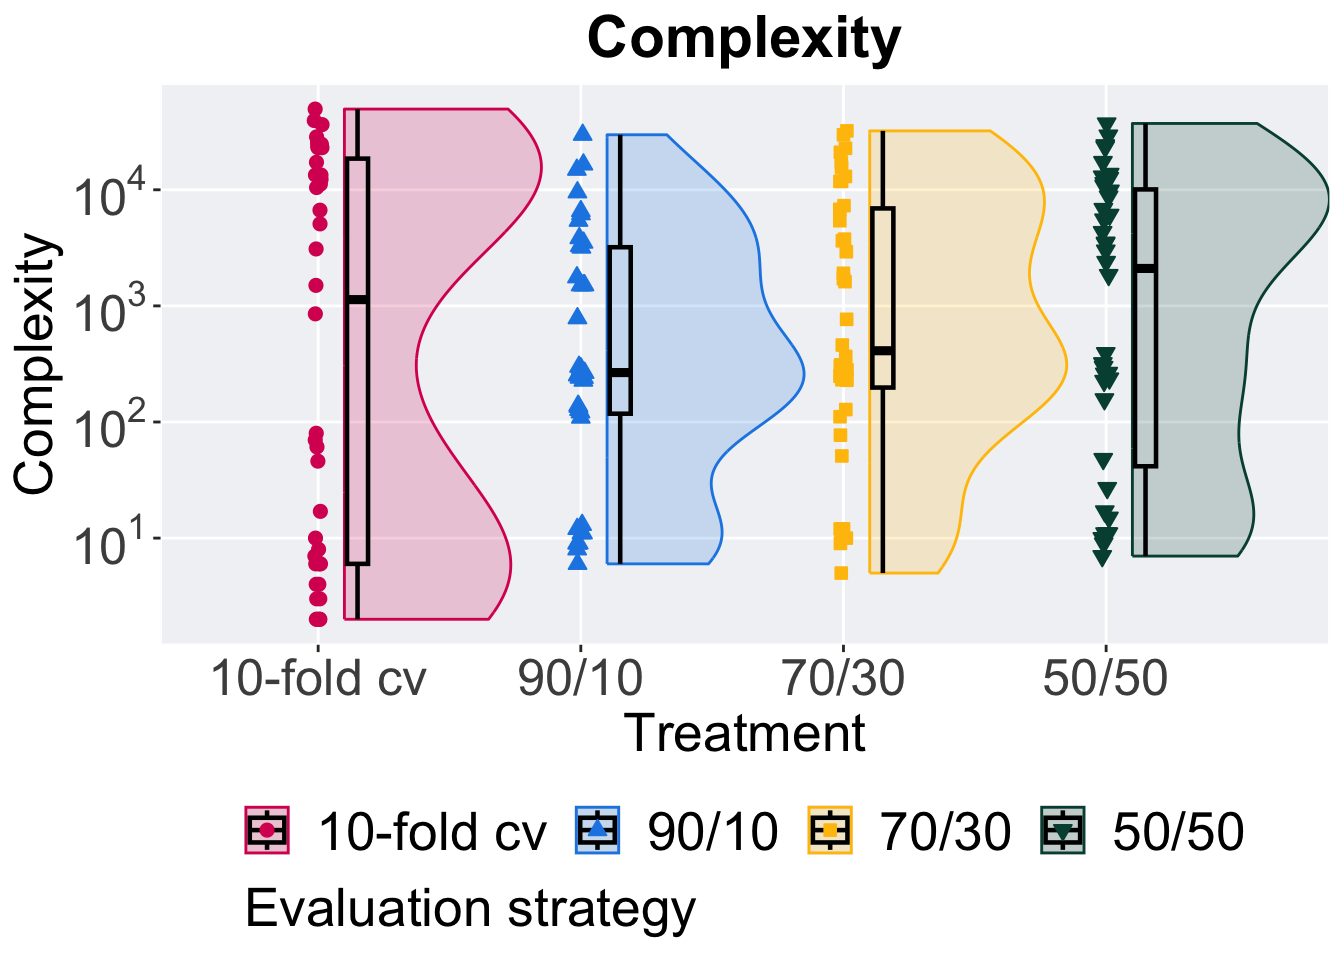
\includegraphics[width=1\linewidth]{lexidate-validation-supplemental_files/figure-latex/com-task-1-plt-1}

Summary statistics for the generation a satisfactory solution is found.

\begin{Shaded}
\begin{Highlighting}[]
\NormalTok{complexity }\OtherTok{\textless{}{-}} \FunctionTok{filter}\NormalTok{(comps, taskid }\SpecialCharTok{==}\NormalTok{ task\_id\_lists[}\DecValTok{1}\NormalTok{])}
\NormalTok{complexity }\SpecialCharTok{\%\textgreater{}\%}
  \FunctionTok{group\_by}\NormalTok{(acro) }\SpecialCharTok{\%\textgreater{}\%}
\NormalTok{  dplyr}\SpecialCharTok{::}\FunctionTok{summarise}\NormalTok{(}
    \AttributeTok{count =} \FunctionTok{n}\NormalTok{(),}
    \AttributeTok{na\_cnt =} \FunctionTok{sum}\NormalTok{(}\FunctionTok{is.na}\NormalTok{(complexity)),}
    \AttributeTok{min =} \FunctionTok{min}\NormalTok{(complexity, }\AttributeTok{na.rm =} \ConstantTok{TRUE}\NormalTok{),}
    \AttributeTok{median =} \FunctionTok{median}\NormalTok{(complexity, }\AttributeTok{na.rm =} \ConstantTok{TRUE}\NormalTok{),}
    \AttributeTok{mean =} \FunctionTok{mean}\NormalTok{(complexity, }\AttributeTok{na.rm =} \ConstantTok{TRUE}\NormalTok{),}
    \AttributeTok{max =} \FunctionTok{max}\NormalTok{(complexity, }\AttributeTok{na.rm =} \ConstantTok{TRUE}\NormalTok{),}
    \AttributeTok{IQR =} \FunctionTok{IQR}\NormalTok{(complexity, }\AttributeTok{na.rm =} \ConstantTok{TRUE}\NormalTok{)}
\NormalTok{  )}
\end{Highlighting}
\end{Shaded}

\begin{verbatim}
## # A tibble: 4 x 8
##   acro       count na_cnt   min median  mean   max    IQR
##   <fct>      <int>  <int> <dbl>  <dbl> <dbl> <dbl>  <dbl>
## 1 10-fold cv    40      0     2  1178  9852. 49555 18698.
## 2 90/10         40      0     6   266. 2825. 29768  3084.
## 3 70/30         40      0     5   414. 5372. 32167  6711.
## 4 50/50         40      0     7  2119  6275. 37256 10039.
\end{verbatim}

Kruskal--Wallis test illustrates evidence of no statistical differences.

\begin{Shaded}
\begin{Highlighting}[]
\FunctionTok{kruskal.test}\NormalTok{(complexity }\SpecialCharTok{\textasciitilde{}}\NormalTok{ acro, }\AttributeTok{data =}\NormalTok{ complexity)}
\end{Highlighting}
\end{Shaded}

\begin{verbatim}
## 
##  Kruskal-Wallis rank sum test
## 
## data:  complexity by acro
## Kruskal-Wallis chi-squared = 2.4209, df = 3, p-value = 0.4898
\end{verbatim}

\hypertarget{task-167184-1}{%
\subsection{Task 167184}\label{task-167184-1}}

\begin{Shaded}
\begin{Highlighting}[]
\FunctionTok{filter}\NormalTok{(comps, taskid }\SpecialCharTok{==}\NormalTok{ task\_id\_lists[}\DecValTok{2}\NormalTok{]) }\SpecialCharTok{\%\textgreater{}\%}
  \FunctionTok{ggplot}\NormalTok{(., }\FunctionTok{aes}\NormalTok{(}\AttributeTok{x =}\NormalTok{ acro, }\AttributeTok{y =}\NormalTok{ complexity, }\AttributeTok{color =}\NormalTok{ acro,}
                \AttributeTok{fill =}\NormalTok{ acro, }\AttributeTok{shape =}\NormalTok{ acro)) }\SpecialCharTok{+}
  \FunctionTok{geom\_flat\_violin}\NormalTok{(}\AttributeTok{position =} \FunctionTok{position\_nudge}\NormalTok{(}\AttributeTok{x =} \FloatTok{0.1}\NormalTok{, }\AttributeTok{y =} \DecValTok{0}\NormalTok{),}
                   \AttributeTok{scale =} \StringTok{"width"}\NormalTok{, }\AttributeTok{alpha =} \FloatTok{0.2}\NormalTok{, }\AttributeTok{width =} \FloatTok{1.5}\NormalTok{) }\SpecialCharTok{+}
  \FunctionTok{geom\_boxplot}\NormalTok{(}\AttributeTok{color =} \StringTok{"black"}\NormalTok{, }\AttributeTok{width =}\NormalTok{ .}\DecValTok{08}\NormalTok{, }\AttributeTok{outlier.shape =} \ConstantTok{NA}\NormalTok{, }\AttributeTok{alpha =} \FloatTok{0.0}\NormalTok{,}
               \AttributeTok{size =} \FloatTok{0.8}\NormalTok{, }\AttributeTok{position =} \FunctionTok{position\_nudge}\NormalTok{(}\AttributeTok{x =}\NormalTok{ .}\DecValTok{15}\NormalTok{, }\AttributeTok{y =} \DecValTok{0}\NormalTok{)) }\SpecialCharTok{+}
  \FunctionTok{geom\_point}\NormalTok{(}\AttributeTok{position =} \FunctionTok{position\_jitter}\NormalTok{(}\AttributeTok{width =}\NormalTok{ .}\DecValTok{015}\NormalTok{, }\AttributeTok{height =}\NormalTok{ .}\DecValTok{0001}\NormalTok{),}
             \AttributeTok{size =} \FloatTok{2.0}\NormalTok{, }\AttributeTok{alpha =} \FloatTok{1.0}\NormalTok{) }\SpecialCharTok{+}
  \FunctionTok{scale\_y\_log10}\NormalTok{(}
    \AttributeTok{name =} \StringTok{"Complexity"}\NormalTok{,}
    \AttributeTok{breaks =} \FunctionTok{trans\_breaks}\NormalTok{(}\StringTok{"log10"}\NormalTok{, }\ControlFlowTok{function}\NormalTok{(x) }\DecValTok{10}\SpecialCharTok{\^{}}\NormalTok{x),}
    \AttributeTok{labels =} \FunctionTok{trans\_format}\NormalTok{(}\StringTok{"log10"}\NormalTok{, }\FunctionTok{math\_format}\NormalTok{(}\DecValTok{10}\SpecialCharTok{\^{}}\NormalTok{.x)),}

\NormalTok{  ) }\SpecialCharTok{+}
  \FunctionTok{scale\_x\_discrete}\NormalTok{(}
    \AttributeTok{name =} \StringTok{"Treatment"}
\NormalTok{  ) }\SpecialCharTok{+}
  \FunctionTok{scale\_shape\_manual}\NormalTok{(}\AttributeTok{values =}\NormalTok{ SHAPE) }\SpecialCharTok{+}
  \FunctionTok{scale\_colour\_manual}\NormalTok{(}\AttributeTok{values =}\NormalTok{ cb\_palette, ) }\SpecialCharTok{+}
  \FunctionTok{scale\_fill\_manual}\NormalTok{(}\AttributeTok{values =}\NormalTok{ cb\_palette) }\SpecialCharTok{+}
  \FunctionTok{ggtitle}\NormalTok{(}\StringTok{"Complexity"}\NormalTok{) }\SpecialCharTok{+}
\NormalTok{  p\_theme }\SpecialCharTok{+}
  \FunctionTok{guides}\NormalTok{(}
    \AttributeTok{shape=}\FunctionTok{guide\_legend}\NormalTok{(}\AttributeTok{nrow =} \DecValTok{1}\NormalTok{, }\AttributeTok{title.position =} \StringTok{"bottom"}\NormalTok{,}
                       \AttributeTok{title =} \StringTok{"Evaluation strategy"}\NormalTok{),}
    \AttributeTok{color=}\FunctionTok{guide\_legend}\NormalTok{(}\AttributeTok{nrow =} \DecValTok{1}\NormalTok{, }\AttributeTok{title.position =} \StringTok{"bottom"}\NormalTok{,}
                       \AttributeTok{title =} \StringTok{"Evaluation strategy"}\NormalTok{),}
    \AttributeTok{fill=}\FunctionTok{guide\_legend}\NormalTok{(}\AttributeTok{nrow =} \DecValTok{1}\NormalTok{, }\AttributeTok{title.position =} \StringTok{"bottom"}\NormalTok{,}
                      \AttributeTok{title =} \StringTok{"Evaluation strategy"}\NormalTok{)}
\NormalTok{  )}
\end{Highlighting}
\end{Shaded}

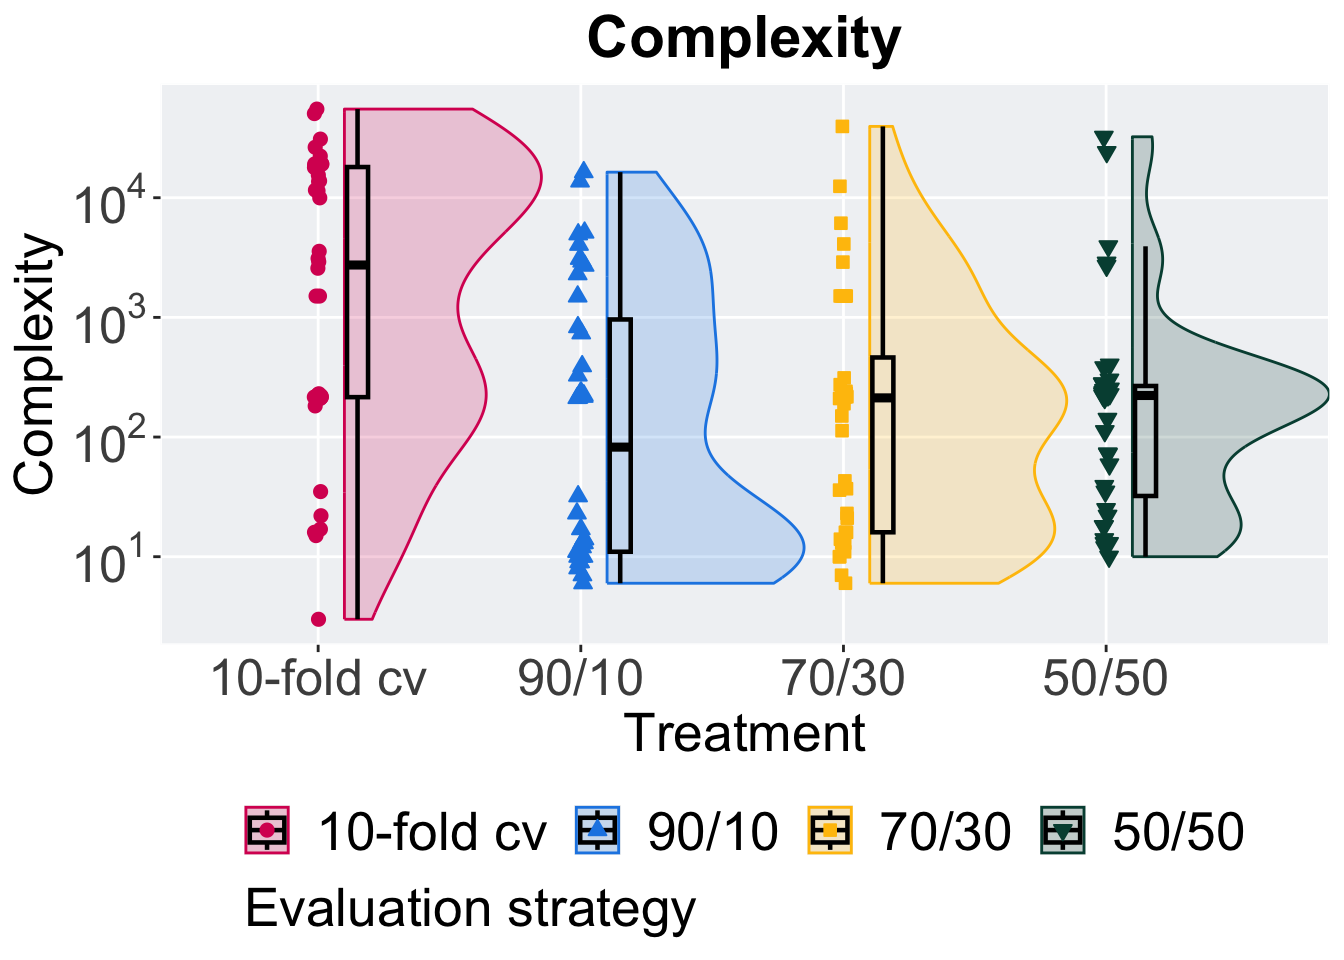
\includegraphics[width=1\linewidth]{lexidate-validation-supplemental_files/figure-latex/com-task-2-plt-1}

Summary statistics for the generation a satisfactory solution is found.

\begin{Shaded}
\begin{Highlighting}[]
\NormalTok{complexity }\OtherTok{\textless{}{-}} \FunctionTok{filter}\NormalTok{(comps, taskid }\SpecialCharTok{==}\NormalTok{ task\_id\_lists[}\DecValTok{2}\NormalTok{])}
\NormalTok{complexity }\SpecialCharTok{\%\textgreater{}\%}
  \FunctionTok{group\_by}\NormalTok{(acro) }\SpecialCharTok{\%\textgreater{}\%}
\NormalTok{  dplyr}\SpecialCharTok{::}\FunctionTok{summarise}\NormalTok{(}
    \AttributeTok{count =} \FunctionTok{n}\NormalTok{(),}
    \AttributeTok{na\_cnt =} \FunctionTok{sum}\NormalTok{(}\FunctionTok{is.na}\NormalTok{(complexity)),}
    \AttributeTok{min =} \FunctionTok{min}\NormalTok{(complexity, }\AttributeTok{na.rm =} \ConstantTok{TRUE}\NormalTok{),}
    \AttributeTok{median =} \FunctionTok{median}\NormalTok{(complexity, }\AttributeTok{na.rm =} \ConstantTok{TRUE}\NormalTok{),}
    \AttributeTok{mean =} \FunctionTok{mean}\NormalTok{(complexity, }\AttributeTok{na.rm =} \ConstantTok{TRUE}\NormalTok{),}
    \AttributeTok{max =} \FunctionTok{max}\NormalTok{(complexity, }\AttributeTok{na.rm =} \ConstantTok{TRUE}\NormalTok{),}
    \AttributeTok{IQR =} \FunctionTok{IQR}\NormalTok{(complexity, }\AttributeTok{na.rm =} \ConstantTok{TRUE}\NormalTok{)}
\NormalTok{  )}
\end{Highlighting}
\end{Shaded}

\begin{verbatim}
## # A tibble: 4 x 8
##   acro       count na_cnt   min median  mean   max    IQR
##   <fct>      <int>  <int> <dbl>  <dbl> <dbl> <dbl>  <dbl>
## 1 10-fold cv    40      0     3  2746. 9800. 55067 17839 
## 2 90/10         40      0     6   122  1513. 16357   985.
## 3 70/30         40      0     6   212. 1898. 39455   594.
## 4 50/50         40      0    10   222. 1780. 32307   235.
\end{verbatim}

Kruskal--Wallis test illustrates evidence of statistical differences.

\begin{Shaded}
\begin{Highlighting}[]
\FunctionTok{kruskal.test}\NormalTok{(complexity }\SpecialCharTok{\textasciitilde{}}\NormalTok{ acro, }\AttributeTok{data =}\NormalTok{ complexity)}
\end{Highlighting}
\end{Shaded}

\begin{verbatim}
## 
##  Kruskal-Wallis rank sum test
## 
## data:  complexity by acro
## Kruskal-Wallis chi-squared = 19.375, df = 3, p-value = 0.0002287
\end{verbatim}

Results for post-hoc Wilcoxon rank-sum test with a Bonferroni correction.

\begin{Shaded}
\begin{Highlighting}[]
\FunctionTok{pairwise.wilcox.test}\NormalTok{(}\AttributeTok{x =}\NormalTok{ complexity}\SpecialCharTok{$}\NormalTok{complexity, }\AttributeTok{g =}\NormalTok{ complexity}\SpecialCharTok{$}\NormalTok{acro,}
                     \AttributeTok{p.adjust.method =} \StringTok{"bonferroni"}\NormalTok{,}
                     \AttributeTok{paired =} \ConstantTok{FALSE}\NormalTok{, }\AttributeTok{conf.int =} \ConstantTok{FALSE}\NormalTok{, }\AttributeTok{alternative =} \StringTok{"l"}\NormalTok{)}
\end{Highlighting}
\end{Shaded}

\begin{verbatim}
## 
##  Pairwise comparisons using Wilcoxon rank sum test with continuity correction 
## 
## data:  complexity$complexity and complexity$acro 
## 
##       10-fold cv 90/10   70/30  
## 90/10 0.00036    -       -      
## 70/30 0.00117    1.00000 -      
## 50/50 0.00742    1.00000 1.00000
## 
## P value adjustment method: bonferroni
\end{verbatim}

\hypertarget{task-167168-1}{%
\subsection{Task 167168}\label{task-167168-1}}

\begin{Shaded}
\begin{Highlighting}[]
\FunctionTok{filter}\NormalTok{(comps, taskid }\SpecialCharTok{==}\NormalTok{ task\_id\_lists[}\DecValTok{3}\NormalTok{]) }\SpecialCharTok{\%\textgreater{}\%}
  \FunctionTok{ggplot}\NormalTok{(., }\FunctionTok{aes}\NormalTok{(}\AttributeTok{x =}\NormalTok{ acro, }\AttributeTok{y =}\NormalTok{ complexity, }\AttributeTok{color =}\NormalTok{ acro,}
                \AttributeTok{fill =}\NormalTok{ acro, }\AttributeTok{shape =}\NormalTok{ acro)) }\SpecialCharTok{+}
  \FunctionTok{geom\_flat\_violin}\NormalTok{(}\AttributeTok{position =} \FunctionTok{position\_nudge}\NormalTok{(}\AttributeTok{x =} \FloatTok{0.1}\NormalTok{, }\AttributeTok{y =} \DecValTok{0}\NormalTok{),}
                   \AttributeTok{scale =} \StringTok{"width"}\NormalTok{, }\AttributeTok{alpha =} \FloatTok{0.2}\NormalTok{, }\AttributeTok{width =} \FloatTok{1.5}\NormalTok{) }\SpecialCharTok{+}
  \FunctionTok{geom\_boxplot}\NormalTok{(}\AttributeTok{color =} \StringTok{"black"}\NormalTok{, }\AttributeTok{width =}\NormalTok{ .}\DecValTok{08}\NormalTok{, }\AttributeTok{outlier.shape =} \ConstantTok{NA}\NormalTok{, }\AttributeTok{alpha =} \FloatTok{0.0}\NormalTok{,}
               \AttributeTok{size =} \FloatTok{0.8}\NormalTok{, }\AttributeTok{position =} \FunctionTok{position\_nudge}\NormalTok{(}\AttributeTok{x =}\NormalTok{ .}\DecValTok{15}\NormalTok{, }\AttributeTok{y =} \DecValTok{0}\NormalTok{)) }\SpecialCharTok{+}
  \FunctionTok{geom\_point}\NormalTok{(}\AttributeTok{position =} \FunctionTok{position\_jitter}\NormalTok{(}\AttributeTok{width =}\NormalTok{ .}\DecValTok{015}\NormalTok{, }\AttributeTok{height =}\NormalTok{ .}\DecValTok{0001}\NormalTok{),}
             \AttributeTok{size =} \FloatTok{2.0}\NormalTok{, }\AttributeTok{alpha =} \FloatTok{1.0}\NormalTok{) }\SpecialCharTok{+}
  \FunctionTok{scale\_y\_log10}\NormalTok{(}
    \AttributeTok{name =} \StringTok{"Complexity"}\NormalTok{,}
    \AttributeTok{breaks =} \FunctionTok{trans\_breaks}\NormalTok{(}\StringTok{"log10"}\NormalTok{, }\ControlFlowTok{function}\NormalTok{(x) }\DecValTok{10}\SpecialCharTok{\^{}}\NormalTok{x),}
    \AttributeTok{labels =} \FunctionTok{trans\_format}\NormalTok{(}\StringTok{"log10"}\NormalTok{, }\FunctionTok{math\_format}\NormalTok{(}\DecValTok{10}\SpecialCharTok{\^{}}\NormalTok{.x)),}
\NormalTok{  ) }\SpecialCharTok{+}
  \FunctionTok{scale\_x\_discrete}\NormalTok{(}
    \AttributeTok{name =} \StringTok{"Treatment"}
\NormalTok{  ) }\SpecialCharTok{+}
  \FunctionTok{scale\_shape\_manual}\NormalTok{(}\AttributeTok{values =}\NormalTok{ SHAPE) }\SpecialCharTok{+}
  \FunctionTok{scale\_colour\_manual}\NormalTok{(}\AttributeTok{values =}\NormalTok{ cb\_palette, ) }\SpecialCharTok{+}
  \FunctionTok{scale\_fill\_manual}\NormalTok{(}\AttributeTok{values =}\NormalTok{ cb\_palette) }\SpecialCharTok{+}
  \FunctionTok{ggtitle}\NormalTok{(}\StringTok{"Complexity"}\NormalTok{) }\SpecialCharTok{+}
\NormalTok{  p\_theme}
\end{Highlighting}
\end{Shaded}

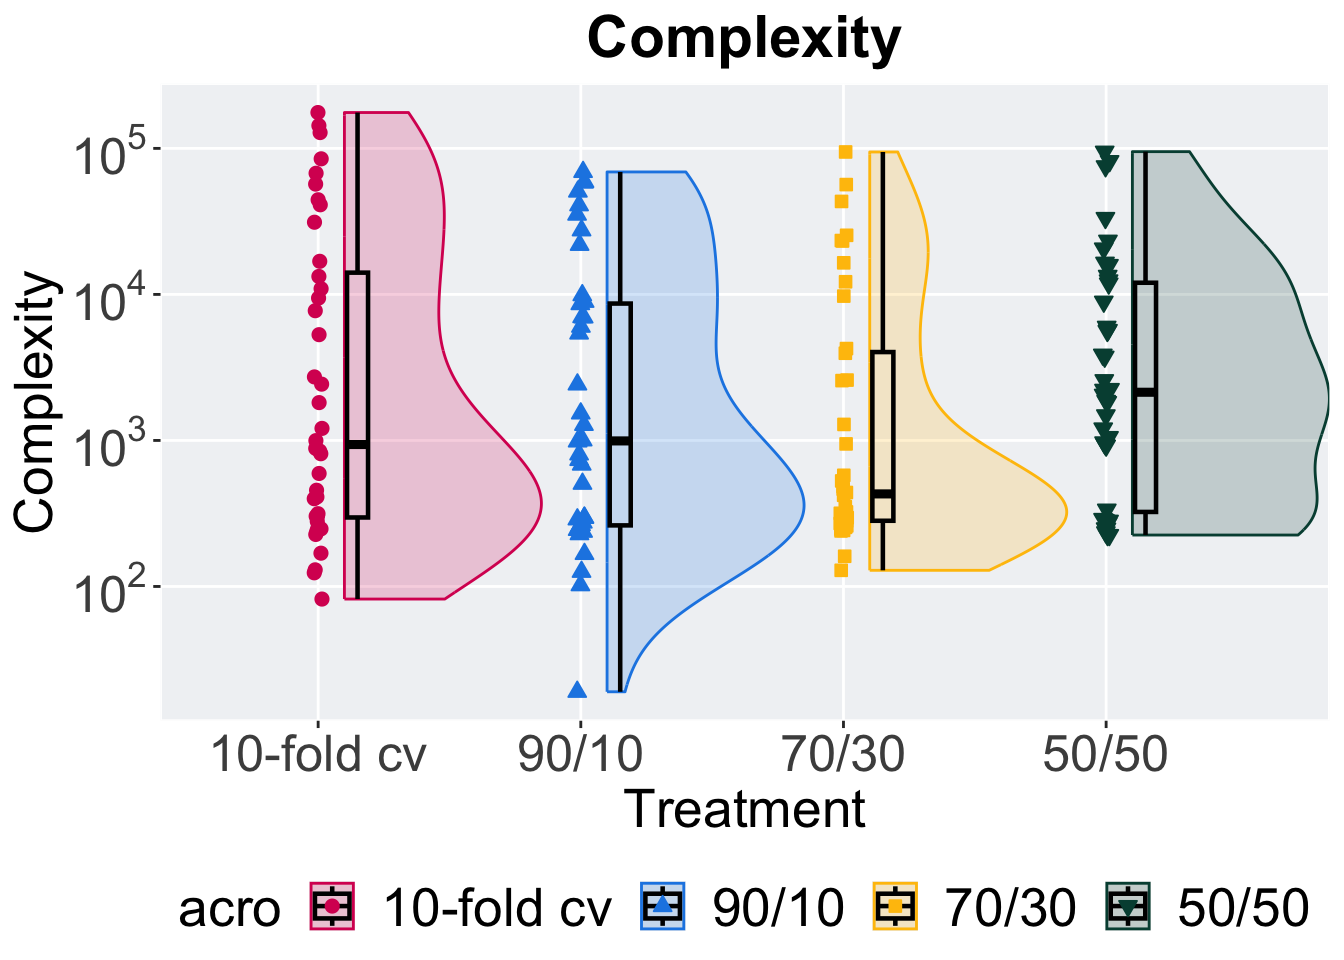
\includegraphics[width=1\linewidth]{lexidate-validation-supplemental_files/figure-latex/com-task-3-plt-1}

Summary statistics for the generation a satisfactory solution is found.

\begin{Shaded}
\begin{Highlighting}[]
\NormalTok{complexity }\OtherTok{\textless{}{-}} \FunctionTok{filter}\NormalTok{(comps, taskid }\SpecialCharTok{==}\NormalTok{ task\_id\_lists[}\DecValTok{3}\NormalTok{])}
\NormalTok{complexity }\SpecialCharTok{\%\textgreater{}\%}
  \FunctionTok{group\_by}\NormalTok{(acro) }\SpecialCharTok{\%\textgreater{}\%}
\NormalTok{  dplyr}\SpecialCharTok{::}\FunctionTok{summarise}\NormalTok{(}
    \AttributeTok{count =} \FunctionTok{n}\NormalTok{(),}
    \AttributeTok{na\_cnt =} \FunctionTok{sum}\NormalTok{(}\FunctionTok{is.na}\NormalTok{(complexity)),}
    \AttributeTok{min =} \FunctionTok{min}\NormalTok{(complexity, }\AttributeTok{na.rm =} \ConstantTok{TRUE}\NormalTok{),}
    \AttributeTok{median =} \FunctionTok{median}\NormalTok{(complexity, }\AttributeTok{na.rm =} \ConstantTok{TRUE}\NormalTok{),}
    \AttributeTok{mean =} \FunctionTok{mean}\NormalTok{(complexity, }\AttributeTok{na.rm =} \ConstantTok{TRUE}\NormalTok{),}
    \AttributeTok{max =} \FunctionTok{max}\NormalTok{(complexity, }\AttributeTok{na.rm =} \ConstantTok{TRUE}\NormalTok{),}
    \AttributeTok{IQR =} \FunctionTok{IQR}\NormalTok{(complexity, }\AttributeTok{na.rm =} \ConstantTok{TRUE}\NormalTok{)}
\NormalTok{  )}
\end{Highlighting}
\end{Shaded}

\begin{verbatim}
## # A tibble: 4 x 8
##   acro       count na_cnt   min median   mean    max    IQR
##   <fct>      <int>  <int> <dbl>  <dbl>  <dbl>  <dbl>  <dbl>
## 1 10-fold cv    40      0    82   940. 21344. 176015 13874.
## 2 90/10         40      0    19   992. 10726.  68977  8396.
## 3 70/30         40      0   129   430.  8209.  94505  3750.
## 4 50/50         40      0   225  2140. 11399.  94975 11698.
\end{verbatim}

Kruskal--Wallis test illustrates evidence of no statistical differences.

\begin{Shaded}
\begin{Highlighting}[]
\FunctionTok{kruskal.test}\NormalTok{(complexity }\SpecialCharTok{\textasciitilde{}}\NormalTok{ acro, }\AttributeTok{data =}\NormalTok{ complexity)}
\end{Highlighting}
\end{Shaded}

\begin{verbatim}
## 
##  Kruskal-Wallis rank sum test
## 
## data:  complexity by acro
## Kruskal-Wallis chi-squared = 3.0019, df = 3, p-value = 0.3913
\end{verbatim}

\hypertarget{task-167161-1}{%
\subsection{Task 167161}\label{task-167161-1}}

\begin{Shaded}
\begin{Highlighting}[]
\FunctionTok{filter}\NormalTok{(comps, taskid }\SpecialCharTok{==}\NormalTok{ task\_id\_lists[}\DecValTok{4}\NormalTok{]) }\SpecialCharTok{\%\textgreater{}\%}
  \FunctionTok{ggplot}\NormalTok{(., }\FunctionTok{aes}\NormalTok{(}\AttributeTok{x =}\NormalTok{ acro, }\AttributeTok{y =}\NormalTok{ complexity, }\AttributeTok{color =}\NormalTok{ acro,}
                \AttributeTok{fill =}\NormalTok{ acro, }\AttributeTok{shape =}\NormalTok{ acro)) }\SpecialCharTok{+}
  \FunctionTok{geom\_flat\_violin}\NormalTok{(}\AttributeTok{position =} \FunctionTok{position\_nudge}\NormalTok{(}\AttributeTok{x =} \FloatTok{0.1}\NormalTok{, }\AttributeTok{y =} \DecValTok{0}\NormalTok{),}
                   \AttributeTok{scale =} \StringTok{"width"}\NormalTok{, }\AttributeTok{alpha =} \FloatTok{0.2}\NormalTok{, }\AttributeTok{width =} \FloatTok{1.5}\NormalTok{) }\SpecialCharTok{+}
  \FunctionTok{geom\_boxplot}\NormalTok{(}\AttributeTok{color =} \StringTok{"black"}\NormalTok{, }\AttributeTok{width =}\NormalTok{ .}\DecValTok{08}\NormalTok{, }\AttributeTok{outlier.shape =} \ConstantTok{NA}\NormalTok{, }\AttributeTok{alpha =} \FloatTok{0.0}\NormalTok{,}
               \AttributeTok{size =} \FloatTok{0.8}\NormalTok{, }\AttributeTok{position =} \FunctionTok{position\_nudge}\NormalTok{(}\AttributeTok{x =}\NormalTok{ .}\DecValTok{15}\NormalTok{, }\AttributeTok{y =} \DecValTok{0}\NormalTok{)) }\SpecialCharTok{+}
  \FunctionTok{geom\_point}\NormalTok{(}\AttributeTok{position =} \FunctionTok{position\_jitter}\NormalTok{(}\AttributeTok{width =}\NormalTok{ .}\DecValTok{015}\NormalTok{, }\AttributeTok{height =}\NormalTok{ .}\DecValTok{0001}\NormalTok{),}
             \AttributeTok{size =} \FloatTok{2.0}\NormalTok{, }\AttributeTok{alpha =} \FloatTok{1.0}\NormalTok{) }\SpecialCharTok{+}
  \FunctionTok{scale\_y\_log10}\NormalTok{(}
    \AttributeTok{name =} \StringTok{"Complexity"}\NormalTok{,}
    \AttributeTok{breaks =} \FunctionTok{trans\_breaks}\NormalTok{(}\StringTok{"log10"}\NormalTok{, }\ControlFlowTok{function}\NormalTok{(x) }\DecValTok{10}\SpecialCharTok{\^{}}\NormalTok{x),}
    \AttributeTok{labels =} \FunctionTok{trans\_format}\NormalTok{(}\StringTok{"log10"}\NormalTok{, }\FunctionTok{math\_format}\NormalTok{(}\DecValTok{10}\SpecialCharTok{\^{}}\NormalTok{.x)),}

\NormalTok{  ) }\SpecialCharTok{+}
  \FunctionTok{scale\_x\_discrete}\NormalTok{(}
    \AttributeTok{name =} \StringTok{"Treatment"}
\NormalTok{  ) }\SpecialCharTok{+}
  \FunctionTok{scale\_shape\_manual}\NormalTok{(}\AttributeTok{values =}\NormalTok{ SHAPE) }\SpecialCharTok{+}
  \FunctionTok{scale\_colour\_manual}\NormalTok{(}\AttributeTok{values =}\NormalTok{ cb\_palette, ) }\SpecialCharTok{+}
  \FunctionTok{scale\_fill\_manual}\NormalTok{(}\AttributeTok{values =}\NormalTok{ cb\_palette) }\SpecialCharTok{+}
  \FunctionTok{ggtitle}\NormalTok{(}\StringTok{"Complexity"}\NormalTok{) }\SpecialCharTok{+}
\NormalTok{  p\_theme }\SpecialCharTok{+}
  \FunctionTok{guides}\NormalTok{(}
    \AttributeTok{shape=}\FunctionTok{guide\_legend}\NormalTok{(}\AttributeTok{nrow =} \DecValTok{1}\NormalTok{, }\AttributeTok{title.position =} \StringTok{"bottom"}\NormalTok{,}
                       \AttributeTok{title =} \StringTok{"Evaluation strategy"}\NormalTok{),}
    \AttributeTok{color=}\FunctionTok{guide\_legend}\NormalTok{(}\AttributeTok{nrow =} \DecValTok{1}\NormalTok{, }\AttributeTok{title.position =} \StringTok{"bottom"}\NormalTok{,}
                       \AttributeTok{title =} \StringTok{"Evaluation strategy"}\NormalTok{),}
    \AttributeTok{fill=}\FunctionTok{guide\_legend}\NormalTok{(}\AttributeTok{nrow =} \DecValTok{1}\NormalTok{, }\AttributeTok{title.position =} \StringTok{"bottom"}\NormalTok{,}
                      \AttributeTok{title =} \StringTok{"Evaluation strategy"}\NormalTok{)}
\NormalTok{  )}
\end{Highlighting}
\end{Shaded}

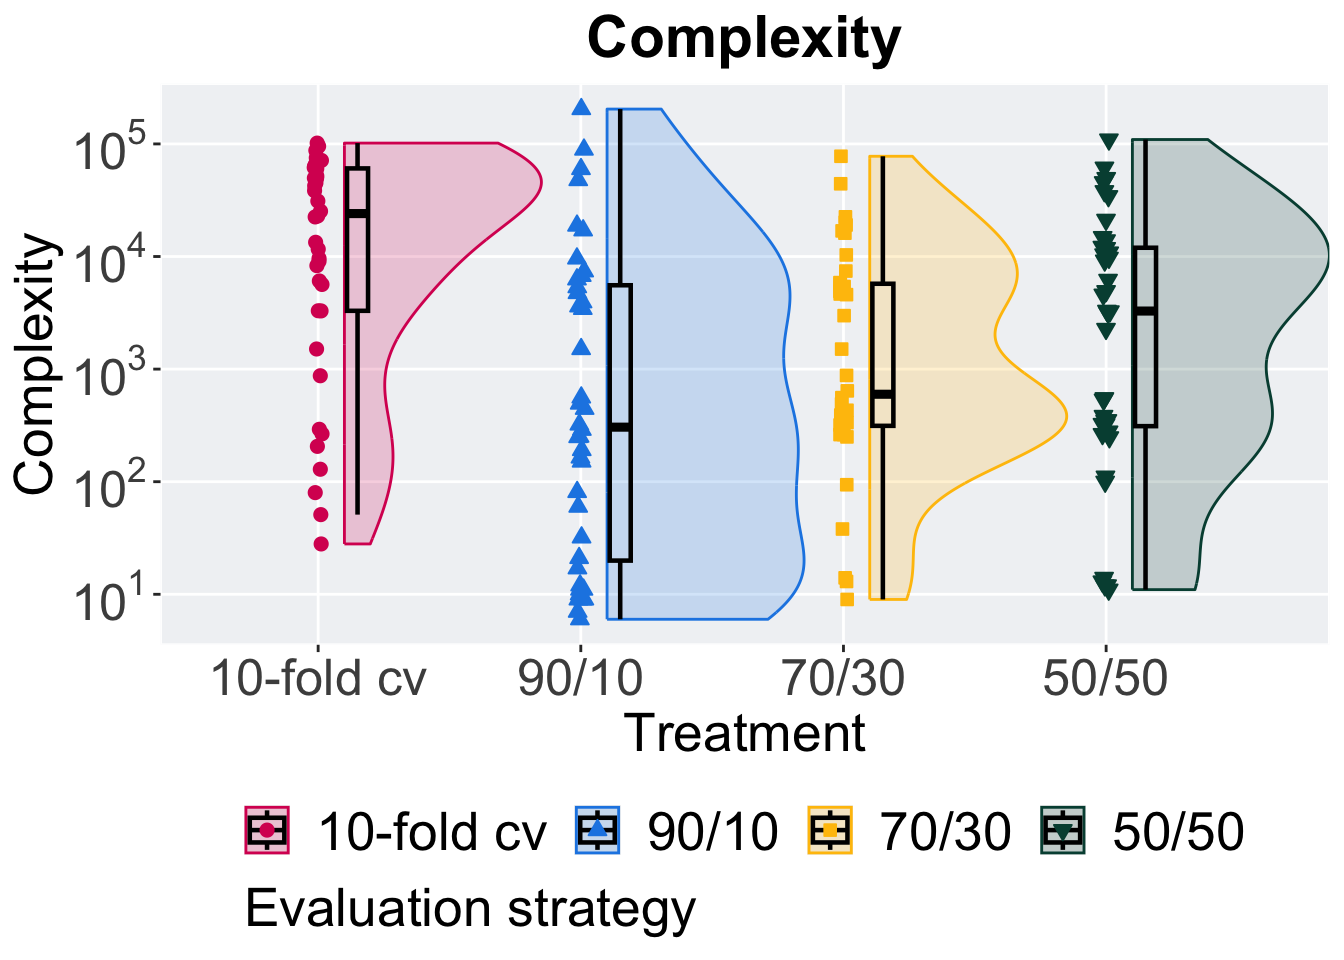
\includegraphics[width=1\linewidth]{lexidate-validation-supplemental_files/figure-latex/com-task-4-plt-1}

Summary statistics for the generation a satisfactory solution is found.

\begin{Shaded}
\begin{Highlighting}[]
\NormalTok{complexity }\OtherTok{\textless{}{-}} \FunctionTok{filter}\NormalTok{(comps, taskid }\SpecialCharTok{==}\NormalTok{ task\_id\_lists[}\DecValTok{4}\NormalTok{])}
\NormalTok{complexity }\SpecialCharTok{\%\textgreater{}\%}
  \FunctionTok{group\_by}\NormalTok{(acro) }\SpecialCharTok{\%\textgreater{}\%}
\NormalTok{  dplyr}\SpecialCharTok{::}\FunctionTok{summarise}\NormalTok{(}
    \AttributeTok{count =} \FunctionTok{n}\NormalTok{(),}
    \AttributeTok{na\_cnt =} \FunctionTok{sum}\NormalTok{(}\FunctionTok{is.na}\NormalTok{(complexity)),}
    \AttributeTok{min =} \FunctionTok{min}\NormalTok{(complexity, }\AttributeTok{na.rm =} \ConstantTok{TRUE}\NormalTok{),}
    \AttributeTok{median =} \FunctionTok{median}\NormalTok{(complexity, }\AttributeTok{na.rm =} \ConstantTok{TRUE}\NormalTok{),}
    \AttributeTok{mean =} \FunctionTok{mean}\NormalTok{(complexity, }\AttributeTok{na.rm =} \ConstantTok{TRUE}\NormalTok{),}
    \AttributeTok{max =} \FunctionTok{max}\NormalTok{(complexity, }\AttributeTok{na.rm =} \ConstantTok{TRUE}\NormalTok{),}
    \AttributeTok{IQR =} \FunctionTok{IQR}\NormalTok{(complexity, }\AttributeTok{na.rm =} \ConstantTok{TRUE}\NormalTok{)}
\NormalTok{  )}
\end{Highlighting}
\end{Shaded}

\begin{verbatim}
## # A tibble: 4 x 8
##   acro       count na_cnt   min median   mean    max    IQR
##   <fct>      <int>  <int> <dbl>  <dbl>  <dbl>  <dbl>  <dbl>
## 1 10-fold cv    40      0    28 24090. 32974. 101704 57312.
## 2 90/10         40      0     6   306. 12308. 203928  5550.
## 3 70/30         40      0     9   600.  7058.  77688  5416 
## 4 50/50         40      0    11  3278. 12379. 109417 11654.
\end{verbatim}

Kruskal--Wallis test illustrates evidence of statistical differences.

\begin{Shaded}
\begin{Highlighting}[]
\FunctionTok{kruskal.test}\NormalTok{(complexity }\SpecialCharTok{\textasciitilde{}}\NormalTok{ acro, }\AttributeTok{data =}\NormalTok{ complexity)}
\end{Highlighting}
\end{Shaded}

\begin{verbatim}
## 
##  Kruskal-Wallis rank sum test
## 
## data:  complexity by acro
## Kruskal-Wallis chi-squared = 25.893, df = 3, p-value = 1.004e-05
\end{verbatim}

Results for post-hoc Wilcoxon rank-sum test with a Bonferroni correction.

\begin{Shaded}
\begin{Highlighting}[]
\FunctionTok{pairwise.wilcox.test}\NormalTok{(}\AttributeTok{x =}\NormalTok{ complexity}\SpecialCharTok{$}\NormalTok{complexity, }\AttributeTok{g =}\NormalTok{ complexity}\SpecialCharTok{$}\NormalTok{acro,}
                     \AttributeTok{p.adjust.method =} \StringTok{"bonferroni"}\NormalTok{,}
                     \AttributeTok{paired =} \ConstantTok{FALSE}\NormalTok{, }\AttributeTok{conf.int =} \ConstantTok{FALSE}\NormalTok{, }\AttributeTok{alternative =} \StringTok{"l"}\NormalTok{)}
\end{Highlighting}
\end{Shaded}

\begin{verbatim}
## 
##  Pairwise comparisons using Wilcoxon rank sum test with continuity correction 
## 
## data:  complexity$complexity and complexity$acro 
## 
##       10-fold cv 90/10   70/30  
## 90/10 4e-05      -       -      
## 70/30 0.00029    1.00000 -      
## 50/50 0.00574    1.00000 1.00000
## 
## P value adjustment method: bonferroni
\end{verbatim}

\hypertarget{task-167185-1}{%
\subsection{Task 167185}\label{task-167185-1}}

\begin{Shaded}
\begin{Highlighting}[]
\FunctionTok{filter}\NormalTok{(comps, taskid }\SpecialCharTok{==}\NormalTok{ task\_id\_lists[}\DecValTok{5}\NormalTok{]) }\SpecialCharTok{\%\textgreater{}\%}
  \FunctionTok{ggplot}\NormalTok{(., }\FunctionTok{aes}\NormalTok{(}\AttributeTok{x =}\NormalTok{ acro, }\AttributeTok{y =}\NormalTok{ complexity, }\AttributeTok{color =}\NormalTok{ acro,}
                \AttributeTok{fill =}\NormalTok{ acro, }\AttributeTok{shape =}\NormalTok{ acro)) }\SpecialCharTok{+}
  \FunctionTok{geom\_flat\_violin}\NormalTok{(}\AttributeTok{position =} \FunctionTok{position\_nudge}\NormalTok{(}\AttributeTok{x =} \FloatTok{0.1}\NormalTok{, }\AttributeTok{y =} \DecValTok{0}\NormalTok{),}
                   \AttributeTok{scale =} \StringTok{"width"}\NormalTok{, }\AttributeTok{alpha =} \FloatTok{0.2}\NormalTok{, }\AttributeTok{width =} \FloatTok{1.5}\NormalTok{) }\SpecialCharTok{+}
  \FunctionTok{geom\_boxplot}\NormalTok{(}\AttributeTok{color =} \StringTok{"black"}\NormalTok{, }\AttributeTok{width =}\NormalTok{ .}\DecValTok{08}\NormalTok{, }\AttributeTok{outlier.shape =} \ConstantTok{NA}\NormalTok{, }\AttributeTok{alpha =} \FloatTok{0.0}\NormalTok{,}
               \AttributeTok{size =} \FloatTok{0.8}\NormalTok{, }\AttributeTok{position =} \FunctionTok{position\_nudge}\NormalTok{(}\AttributeTok{x =}\NormalTok{ .}\DecValTok{15}\NormalTok{, }\AttributeTok{y =} \DecValTok{0}\NormalTok{)) }\SpecialCharTok{+}
  \FunctionTok{geom\_point}\NormalTok{(}\AttributeTok{position =} \FunctionTok{position\_jitter}\NormalTok{(}\AttributeTok{width =}\NormalTok{ .}\DecValTok{015}\NormalTok{, }\AttributeTok{height =}\NormalTok{ .}\DecValTok{0001}\NormalTok{),}
             \AttributeTok{size =} \FloatTok{2.0}\NormalTok{, }\AttributeTok{alpha =} \FloatTok{1.0}\NormalTok{) }\SpecialCharTok{+}
  \FunctionTok{scale\_y\_log10}\NormalTok{(}
    \AttributeTok{name =} \StringTok{"Complexity"}\NormalTok{,}
    \AttributeTok{breaks =} \FunctionTok{trans\_breaks}\NormalTok{(}\StringTok{"log10"}\NormalTok{, }\ControlFlowTok{function}\NormalTok{(x) }\DecValTok{10}\SpecialCharTok{\^{}}\NormalTok{x),}
    \AttributeTok{labels =} \FunctionTok{trans\_format}\NormalTok{(}\StringTok{"log10"}\NormalTok{, }\FunctionTok{math\_format}\NormalTok{(}\DecValTok{10}\SpecialCharTok{\^{}}\NormalTok{.x)),}
\NormalTok{  ) }\SpecialCharTok{+}
  \FunctionTok{scale\_x\_discrete}\NormalTok{(}
    \AttributeTok{name =} \StringTok{"Treatment"}
\NormalTok{  ) }\SpecialCharTok{+}
  \FunctionTok{scale\_shape\_manual}\NormalTok{(}\AttributeTok{values =}\NormalTok{ SHAPE) }\SpecialCharTok{+}
  \FunctionTok{scale\_colour\_manual}\NormalTok{(}\AttributeTok{values =}\NormalTok{ cb\_palette, ) }\SpecialCharTok{+}
  \FunctionTok{scale\_fill\_manual}\NormalTok{(}\AttributeTok{values =}\NormalTok{ cb\_palette) }\SpecialCharTok{+}
  \FunctionTok{ggtitle}\NormalTok{(}\StringTok{"Complexity"}\NormalTok{) }\SpecialCharTok{+}
\NormalTok{  p\_theme }\SpecialCharTok{+}
  \FunctionTok{guides}\NormalTok{(}
    \AttributeTok{shape=}\FunctionTok{guide\_legend}\NormalTok{(}\AttributeTok{nrow =} \DecValTok{1}\NormalTok{, }\AttributeTok{title.position =} \StringTok{"bottom"}\NormalTok{,}
                       \AttributeTok{title =} \StringTok{"Evaluation strategy"}\NormalTok{),}
    \AttributeTok{color=}\FunctionTok{guide\_legend}\NormalTok{(}\AttributeTok{nrow =} \DecValTok{1}\NormalTok{, }\AttributeTok{title.position =} \StringTok{"bottom"}\NormalTok{,}
                       \AttributeTok{title =} \StringTok{"Evaluation strategy"}\NormalTok{),}
    \AttributeTok{fill=}\FunctionTok{guide\_legend}\NormalTok{(}\AttributeTok{nrow =} \DecValTok{1}\NormalTok{, }\AttributeTok{title.position =} \StringTok{"bottom"}\NormalTok{,}
                      \AttributeTok{title =} \StringTok{"Evaluation strategy"}\NormalTok{)}
\NormalTok{  )}
\end{Highlighting}
\end{Shaded}

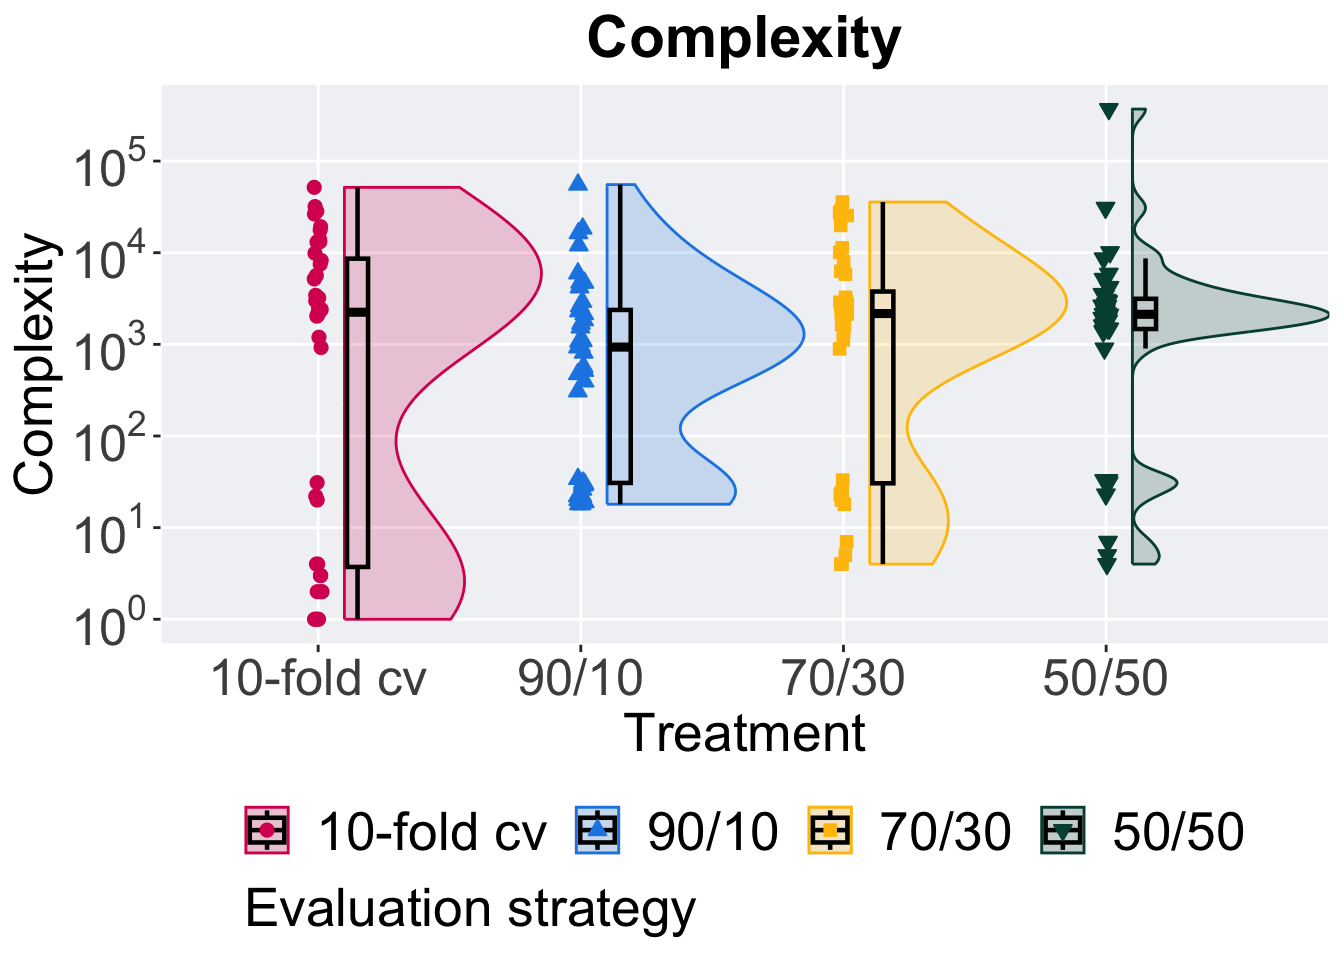
\includegraphics[width=1\linewidth]{lexidate-validation-supplemental_files/figure-latex/com-task-5-plt-1}

Summary statistics for the generation a satisfactory solution is found.

\begin{Shaded}
\begin{Highlighting}[]
\NormalTok{complexity }\OtherTok{\textless{}{-}} \FunctionTok{filter}\NormalTok{(comps, taskid }\SpecialCharTok{==}\NormalTok{ task\_id\_lists[}\DecValTok{5}\NormalTok{])}
\NormalTok{complexity }\SpecialCharTok{\%\textgreater{}\%}
  \FunctionTok{group\_by}\NormalTok{(acro) }\SpecialCharTok{\%\textgreater{}\%}
\NormalTok{  dplyr}\SpecialCharTok{::}\FunctionTok{summarise}\NormalTok{(}
    \AttributeTok{count =} \FunctionTok{n}\NormalTok{(),}
    \AttributeTok{na\_cnt =} \FunctionTok{sum}\NormalTok{(}\FunctionTok{is.na}\NormalTok{(complexity)),}
    \AttributeTok{min =} \FunctionTok{min}\NormalTok{(complexity, }\AttributeTok{na.rm =} \ConstantTok{TRUE}\NormalTok{),}
    \AttributeTok{median =} \FunctionTok{median}\NormalTok{(complexity, }\AttributeTok{na.rm =} \ConstantTok{TRUE}\NormalTok{),}
    \AttributeTok{mean =} \FunctionTok{mean}\NormalTok{(complexity, }\AttributeTok{na.rm =} \ConstantTok{TRUE}\NormalTok{),}
    \AttributeTok{max =} \FunctionTok{max}\NormalTok{(complexity, }\AttributeTok{na.rm =} \ConstantTok{TRUE}\NormalTok{),}
    \AttributeTok{IQR =} \FunctionTok{IQR}\NormalTok{(complexity, }\AttributeTok{na.rm =} \ConstantTok{TRUE}\NormalTok{)}
\NormalTok{  )}
\end{Highlighting}
\end{Shaded}

\begin{verbatim}
## # A tibble: 4 x 8
##   acro       count na_cnt   min median   mean    max   IQR
##   <fct>      <int>  <int> <dbl>  <dbl>  <dbl>  <dbl> <dbl>
## 1 10-fold cv    40      0     1  2244   6931.  51694 8638.
## 2 90/10         40      0    18   934.  3667.  55371 2348.
## 3 70/30         40      0     4  2169   5487.  35738 3874.
## 4 50/50         40      0     4  2127  12314. 369366 1675
\end{verbatim}

Kruskal--Wallis test illustrates evidence of no statistical differences.

\begin{Shaded}
\begin{Highlighting}[]
\FunctionTok{kruskal.test}\NormalTok{(complexity }\SpecialCharTok{\textasciitilde{}}\NormalTok{ acro, }\AttributeTok{data =}\NormalTok{ complexity)}
\end{Highlighting}
\end{Shaded}

\begin{verbatim}
## 
##  Kruskal-Wallis rank sum test
## 
## data:  complexity by acro
## Kruskal-Wallis chi-squared = 3.3929, df = 3, p-value = 0.3349
\end{verbatim}

\hypertarget{task-189905-1}{%
\subsection{Task 189905}\label{task-189905-1}}

\begin{Shaded}
\begin{Highlighting}[]
\FunctionTok{filter}\NormalTok{(comps, taskid }\SpecialCharTok{==}\NormalTok{ task\_id\_lists[}\DecValTok{6}\NormalTok{]) }\SpecialCharTok{\%\textgreater{}\%}
  \FunctionTok{ggplot}\NormalTok{(., }\FunctionTok{aes}\NormalTok{(}\AttributeTok{x =}\NormalTok{ acro, }\AttributeTok{y =}\NormalTok{ complexity, }\AttributeTok{color =}\NormalTok{ acro,}
                \AttributeTok{fill =}\NormalTok{ acro, }\AttributeTok{shape =}\NormalTok{ acro)) }\SpecialCharTok{+}
  \FunctionTok{geom\_flat\_violin}\NormalTok{(}\AttributeTok{position =} \FunctionTok{position\_nudge}\NormalTok{(}\AttributeTok{x =} \FloatTok{0.1}\NormalTok{, }\AttributeTok{y =} \DecValTok{0}\NormalTok{),}
                   \AttributeTok{scale =} \StringTok{"width"}\NormalTok{, }\AttributeTok{alpha =} \FloatTok{0.2}\NormalTok{, }\AttributeTok{width =} \FloatTok{1.5}\NormalTok{) }\SpecialCharTok{+}
  \FunctionTok{geom\_boxplot}\NormalTok{(}\AttributeTok{color =} \StringTok{"black"}\NormalTok{, }\AttributeTok{width =}\NormalTok{ .}\DecValTok{08}\NormalTok{, }\AttributeTok{outlier.shape =} \ConstantTok{NA}\NormalTok{, }\AttributeTok{alpha =} \FloatTok{0.0}\NormalTok{,}
               \AttributeTok{size =} \FloatTok{0.8}\NormalTok{, }\AttributeTok{position =} \FunctionTok{position\_nudge}\NormalTok{(}\AttributeTok{x =}\NormalTok{ .}\DecValTok{15}\NormalTok{, }\AttributeTok{y =} \DecValTok{0}\NormalTok{)) }\SpecialCharTok{+}
  \FunctionTok{geom\_point}\NormalTok{(}\AttributeTok{position =} \FunctionTok{position\_jitter}\NormalTok{(}\AttributeTok{width =}\NormalTok{ .}\DecValTok{015}\NormalTok{, }\AttributeTok{height =}\NormalTok{ .}\DecValTok{0001}\NormalTok{),}
             \AttributeTok{size =} \FloatTok{2.0}\NormalTok{, }\AttributeTok{alpha =} \FloatTok{1.0}\NormalTok{) }\SpecialCharTok{+}
  \FunctionTok{scale\_y\_log10}\NormalTok{(}
    \AttributeTok{name =} \StringTok{"Complexity"}\NormalTok{,}
    \AttributeTok{breaks =} \FunctionTok{trans\_breaks}\NormalTok{(}\StringTok{"log10"}\NormalTok{, }\ControlFlowTok{function}\NormalTok{(x) }\DecValTok{10}\SpecialCharTok{\^{}}\NormalTok{x),}
    \AttributeTok{labels =} \FunctionTok{trans\_format}\NormalTok{(}\StringTok{"log10"}\NormalTok{, }\FunctionTok{math\_format}\NormalTok{(}\DecValTok{10}\SpecialCharTok{\^{}}\NormalTok{.x)),}

\NormalTok{  ) }\SpecialCharTok{+}
  \FunctionTok{scale\_x\_discrete}\NormalTok{(}
    \AttributeTok{name =} \StringTok{"Treatment"}
\NormalTok{  ) }\SpecialCharTok{+}
  \FunctionTok{scale\_shape\_manual}\NormalTok{(}\AttributeTok{values =}\NormalTok{ SHAPE) }\SpecialCharTok{+}
  \FunctionTok{scale\_colour\_manual}\NormalTok{(}\AttributeTok{values =}\NormalTok{ cb\_palette, ) }\SpecialCharTok{+}
  \FunctionTok{scale\_fill\_manual}\NormalTok{(}\AttributeTok{values =}\NormalTok{ cb\_palette) }\SpecialCharTok{+}
  \FunctionTok{ggtitle}\NormalTok{(}\StringTok{"Complexity"}\NormalTok{) }\SpecialCharTok{+}
\NormalTok{  p\_theme }\SpecialCharTok{+}
  \FunctionTok{guides}\NormalTok{(}
    \AttributeTok{shape=}\FunctionTok{guide\_legend}\NormalTok{(}\AttributeTok{nrow =} \DecValTok{1}\NormalTok{, }\AttributeTok{title.position =} \StringTok{"bottom"}\NormalTok{,}
                       \AttributeTok{title =} \StringTok{"Evaluation strategy"}\NormalTok{),}
    \AttributeTok{color=}\FunctionTok{guide\_legend}\NormalTok{(}\AttributeTok{nrow =} \DecValTok{1}\NormalTok{, }\AttributeTok{title.position =} \StringTok{"bottom"}\NormalTok{,}
                       \AttributeTok{title =} \StringTok{"Evaluation strategy"}\NormalTok{),}
    \AttributeTok{fill=}\FunctionTok{guide\_legend}\NormalTok{(}\AttributeTok{nrow =} \DecValTok{1}\NormalTok{, }\AttributeTok{title.position =} \StringTok{"bottom"}\NormalTok{,}
                      \AttributeTok{title =} \StringTok{"Evaluation strategy"}\NormalTok{)}
\NormalTok{  )}
\end{Highlighting}
\end{Shaded}

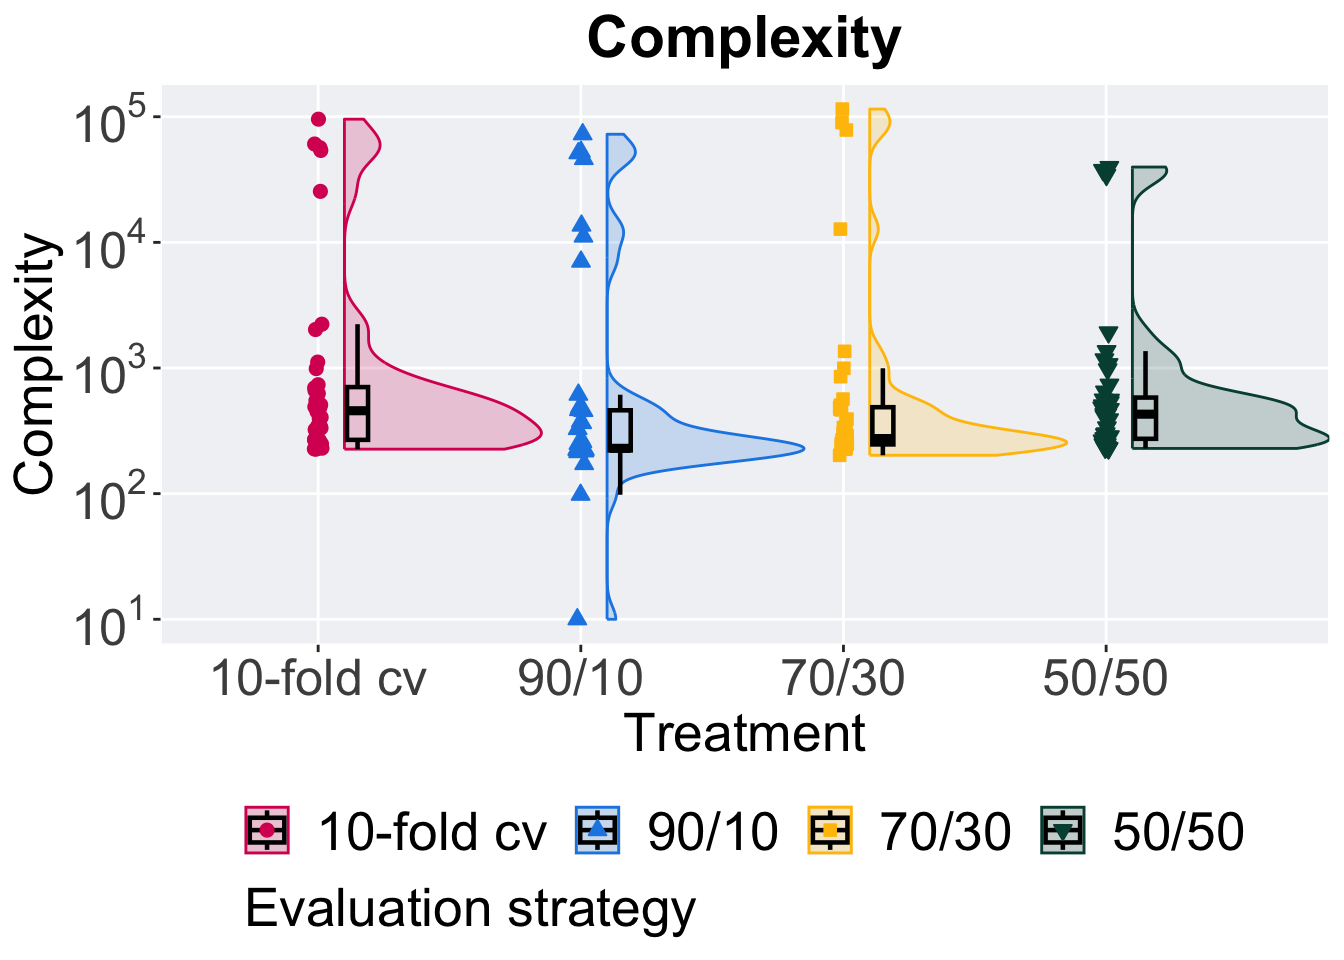
\includegraphics[width=1\linewidth]{lexidate-validation-supplemental_files/figure-latex/com-task-6-plt-1}

Summary statistics for the generation a satisfactory solution is found.

\begin{Shaded}
\begin{Highlighting}[]
\NormalTok{complexity }\OtherTok{\textless{}{-}} \FunctionTok{filter}\NormalTok{(comps, taskid }\SpecialCharTok{==}\NormalTok{ task\_id\_lists[}\DecValTok{6}\NormalTok{])}
\NormalTok{complexity }\SpecialCharTok{\%\textgreater{}\%}
  \FunctionTok{group\_by}\NormalTok{(acro) }\SpecialCharTok{\%\textgreater{}\%}
\NormalTok{  dplyr}\SpecialCharTok{::}\FunctionTok{summarise}\NormalTok{(}
    \AttributeTok{count =} \FunctionTok{n}\NormalTok{(),}
    \AttributeTok{na\_cnt =} \FunctionTok{sum}\NormalTok{(}\FunctionTok{is.na}\NormalTok{(complexity)),}
    \AttributeTok{min =} \FunctionTok{min}\NormalTok{(complexity, }\AttributeTok{na.rm =} \ConstantTok{TRUE}\NormalTok{),}
    \AttributeTok{median =} \FunctionTok{median}\NormalTok{(complexity, }\AttributeTok{na.rm =} \ConstantTok{TRUE}\NormalTok{),}
    \AttributeTok{mean =} \FunctionTok{mean}\NormalTok{(complexity, }\AttributeTok{na.rm =} \ConstantTok{TRUE}\NormalTok{),}
    \AttributeTok{max =} \FunctionTok{max}\NormalTok{(complexity, }\AttributeTok{na.rm =} \ConstantTok{TRUE}\NormalTok{),}
    \AttributeTok{IQR =} \FunctionTok{IQR}\NormalTok{(complexity, }\AttributeTok{na.rm =} \ConstantTok{TRUE}\NormalTok{)}
\NormalTok{  )}
\end{Highlighting}
\end{Shaded}

\begin{verbatim}
## # A tibble: 4 x 8
##   acro       count na_cnt   min median  mean    max   IQR
##   <fct>      <int>  <int> <dbl>  <dbl> <dbl>  <dbl> <dbl>
## 1 10-fold cv    40      0   226   457  7771.  95634  437.
## 2 90/10         40      0    10   230. 6579.  72557  240.
## 3 70/30         40      0   202   274. 7736. 115088  241 
## 4 50/50         40      0   229   429  3262.  39776  310.
\end{verbatim}

Kruskal--Wallis test illustrates evidence of statistical differences.

\begin{Shaded}
\begin{Highlighting}[]
\FunctionTok{kruskal.test}\NormalTok{(complexity }\SpecialCharTok{\textasciitilde{}}\NormalTok{ acro, }\AttributeTok{data =}\NormalTok{ complexity)}
\end{Highlighting}
\end{Shaded}

\begin{verbatim}
## 
##  Kruskal-Wallis rank sum test
## 
## data:  complexity by acro
## Kruskal-Wallis chi-squared = 17.387, df = 3, p-value = 0.0005884
\end{verbatim}

Results for post-hoc Wilcoxon rank-sum test with a Bonferroni correction.

\begin{Shaded}
\begin{Highlighting}[]
\FunctionTok{pairwise.wilcox.test}\NormalTok{(}\AttributeTok{x =}\NormalTok{ complexity}\SpecialCharTok{$}\NormalTok{complexity, }\AttributeTok{g =}\NormalTok{ complexity}\SpecialCharTok{$}\NormalTok{acro,}
                     \AttributeTok{p.adjust.method =} \StringTok{"bonferroni"}\NormalTok{,}
                     \AttributeTok{paired =} \ConstantTok{FALSE}\NormalTok{, }\AttributeTok{conf.int =} \ConstantTok{FALSE}\NormalTok{, }\AttributeTok{alternative =} \StringTok{"l"}\NormalTok{)}
\end{Highlighting}
\end{Shaded}

\begin{verbatim}
## 
##  Pairwise comparisons using Wilcoxon rank sum test with continuity correction 
## 
## data:  complexity$complexity and complexity$acro 
## 
##       10-fold cv 90/10  70/30 
## 90/10 0.0019     -      -     
## 70/30 0.1592     1.0000 -     
## 50/50 1.0000     1.0000 1.0000
## 
## P value adjustment method: bonferroni
\end{verbatim}

  \bibliography{packages.bib,supplemental.bib}

\end{document}
